%% Aide-mémoire
\documentclass[10pt, french]{article}
%% -----------------------------
%% Préambule
%% -----------------------------
\usepackage{xcolor}
\usepackage{bbding}
\usepackage{pifont}
\usepackage{multido}
\def\cours{Modern Actuarial Statistics}
\def\sigle{MAS-I}
\def\session{Avril 2019}
\def\auteur{Nicholas Langevin}
\def\BackgroundColor{white}
% \definecolor{section_color}{rgb}{0.1,0.1,1}
\def\SubSectionColor{blue!30!black}
% !TEX encoding = UTF-8 Unicode
% LaTeX Preamble
% Author : Gabriel Crépeault-Cauchon

% HOW-TO : copy-paste this file in the same directory as your .tex file, and add in your preamble the next command right after you have specified your documentclass : 
% \input{preamble-cheatsht.tex}
% ---------------------------------------------
% ---------------------------------------------

%% -----------------------------
%% Encoding packages
%% -----------------------------
\usepackage[utf8]{inputenc}
\usepackage[T1]{fontenc}
\usepackage{babel}
\usepackage{lmodern}

%% -----------------------------
%% Variable definition
%% -----------------------------


\def\session{Automne 2018}
\def\auteur{Gabriel Crépeault-Cauchon // Nicholas Langevin}
\def\BackgroundColor{white}


%% -----------------------------
%% Margin and layout
%% -----------------------------
% Determine the margin for cheatsheet
\usepackage[landscape, hmargin=1cm, vmargin=1.7cm]{geometry}
\usepackage{multicol}

% Remove automatic indentation after section/subsection title.
\setlength{\parindent}{0cm}

% Save space in cheatsheet by removing space between align environment and normal text.
\usepackage{etoolbox}
\newcommand{\zerodisplayskips}{%
  \setlength{\abovedisplayskip}{0pt}%
  \setlength{\belowdisplayskip}{0pt}%
  \setlength{\abovedisplayshortskip}{0pt}%
  \setlength{\belowdisplayshortskip}{0pt}}
\appto{\normalsize}{\zerodisplayskips}
\appto{\small}{\zerodisplayskips}
\appto{\footnotesize}{\zerodisplayskips}

%% -----------------------------
%% URL and links
%% -----------------------------
\usepackage{hyperref}
\hypersetup{colorlinks = true, urlcolor = gray!70!white, linkcolor = black}

%% -----------------------------
%% Document policy (uncomment only one)
%% -----------------------------
%	\usepackage{concrete}
	\usepackage{mathpazo}
%	\usepackage{frcursive} %% permet d'écrire en lettres attachées
%	\usepackage{aeguill}
%	\usepackage{mathptmx}
%	\usepackage{fourier} 

%% -----------------------------
%% Math configuration
%% -----------------------------
\usepackage[fleqn]{amsmath}
\usepackage{amsthm,amssymb,latexsym,amsfonts}
\usepackage{empheq}
\usepackage{numprint}

% Mathematics shortcut
\newcommand{\reels}{\mathbb{R}}
\newcommand{\entiers}{\mathbb{Z}}
\newcommand{\naturels}{\mathbb{N}}
\newcommand{\eval}{\biggr \rvert}
\usepackage{cancel}
\newcommand{\derivee}[1]{\frac{\partial}{\partial #1}}
\newcommand{\prob}[1]{\Pr \left( #1 \right)}
\newcommand{\esp}[1]{\mathrm{E} \left[ #1 \right]}
\newcommand{\variance}[1]{\mathrm{Var} \left( #1 \right)}
\newcommand{\covar}[1]{\mathrm{Cov} \left( #1 \right)}
\newcommand{\laplace}{\mathcal{L}}

% To indicate equation number on a specific line in align environment
\newcommand\numberthis{\addtocounter{equation}{1}\tag{\theequation}}

% Actuarial notation package
\usepackage{actuarialsymbol}
\usepackage{actuarialangle}

% Matricial anotation for math symbols (\bm{•})
\usepackage{bm}
% matricial notation variable (bold style)
\newcommand{\matr}[1]{\mathbf{#1}}



%% -----------------------------
%% tcolorbox configuration
%% -----------------------------
\usepackage{tcolorbox}
\tcbuselibrary{xparse}
\tcbuselibrary{breakable}

%% Définition boite pour définition
\DeclareTColorBox{definition}{ o }% #1 parameter
{colframe=blue!60!green,colback=blue!5!white, % color of the box
breakable, pad at break*=0mm, % to split the box
title = {#1},
after title = {\large \hfill \faBook}
}

%% -----------------------------
%% Graphics and pictures
%% -----------------------------
\usepackage{graphicx}
\usepackage{pict2e}

%% -----------------------------
%% insert pdf pages into document
%% -----------------------------
\usepackage{pdfpages}

%% -----------------------------
%% Color configuration
%% -----------------------------
\usepackage{color, soulutf8, colortbl}


% New color definition
% Source : http://latexcolor.com


% usefull shortcut for colored text
\newcommand{\orange}{\textcolor{orange}}
\newcommand{\red}{\textcolor{red}}
\newcommand{\cyan}{\textcolor{cyan}}
\newcommand{\blue}{\textcolor{blue}}
\newcommand{\green}{\textcolor{green}}
\newcommand{\purple}{\textcolor{magenta}}
\newcommand{\yellow}{\textcolor{yellow}}


%% -----------------------------
%% Enumerate environment configuration
%% -----------------------------
% Custum enumerate & itemize Package
\usepackage{enumitem}
% French Setup for itemize function
\frenchbsetup{StandardItemLabels=true}
% Change default label for itemize
\renewcommand{\labelitemi}{\faAngleRight}

%% -----------------------------
%% Tabular column type configuration
%% -----------------------------
\newcolumntype{C}{>{$}c<{$}} % math-mode version of "l" column type
\newcolumntype{L}{>{$}l<{$}} % math-mode version of "l" column type
\newcolumntype{R}{>{$}r<{$}} % math-mode version of "l" column type
\newcolumntype{f}{>{\columncolor{green!20!white}}p{1cm}}
% configuration to force a line break within a single cell
\usepackage{makecell}



%% -----------------------------
%% Fontawesome for special symbols
%% -----------------------------
\usepackage{fontawesome}

%% -----------------------------
%% Section Font customization
%% -----------------------------
\usepackage{sectsty}
\sectionfont{\color{\SectionColor}}
\subsectionfont{\color{\SubSectionColor}}

%% -----------------------------
%% Footer/Header Customization
%% -----------------------------
\usepackage{lastpage}
\usepackage{fancyhdr}
\pagestyle{fancy}
% Header
\fancyhead{} 	% Reset
\fancyhead[L]{Aide-mémoire pour~ \cours ~(\textbf{\sigle})}
\fancyhead[R]{\auteur}

% Footer
\fancyfoot{}		% Reset
\fancyfoot[R]{\thepage ~de~ \pageref{LastPage}}
\fancyfoot[L]{\href{https://github.com/gabrielcrepeault/latex-template}{\faGithub \ gabrielcrepeault/latex-template}}

% page background color
\pagecolor{\BackgroundColor}






%% END OF PREAMBLE
% ---------------------------------------------
% ---------------------------------------------
\title{MAS-1 \\ Study Review}
\author{Nicholas Langevin}
%% -----------------------------
%% Début du document
%% -----------------------------
\begin{document}

\maketitle
\vspace{50pt}
\begin{center}
\begin{minipage}[c]{7.5cm}
    \begin{itemize}
        \LARGE
        \item[\color{magenta}\ding{235}] Probability Review
        \item[\color{brown}  \ding{235}] \hyperref[Stochastic Processes]{Stochastic Processes}
        \item[\color{purple} \ding{235}] Life Contingencies
        \item[\color{orange} \ding{235}] Simulation
        \item[\color{red}    \ding{235}] Statistics
        \item[\color{blue}   \ding{235}] Extended Linear Model
        \item[\color{green}  \ding{235}] Time Series
    \end{itemize}
\end{minipage}
\end{center}
\newpage

\small
\begin{multicols*}{3} % Nombre de colonnes (peut être changé plus tard.)
\def\SectionColor{magenta!80!white}
\section*{Lesson 1: Probability Review}
\begin{itemize}[align=left,leftmargin=*]
    \item \textbf{Bernouilli Shortcut:} If a random variable can only assume two values $a$ and $b$ with probability $q$ and $1-q$, then is variance is \\ $q(1-q)(b-a)^2$
\end{itemize}

\section*{Lesson 2: Parametric Distributions}
\begin{itemize}[align=left,leftmargin=*]
    \item \textbf{Transformations:}
    \begin{itemize}
        \item Transformed: $\tau > 0$
        \item Inverse: $\tau = -1$
        \item Inverse-Transformed: $\tau < 0, \tau \neq 1$
    \end{itemize}
\end{itemize}

\def\SectionColor{brown!80!white}
\section*{Lesson 4: Markov Chains}
\begin{itemize}[align=left,leftmargin=*]
    \item \textbf{Chapman-Kolmogorov:} \[ P_{ij}^{(n+m)} = \sum_{k=0}^\infty P_{ik}^{(n)}  P_{kj}^{(m)} \]
    \item \textbf{Gambler's ruin:} Let N the target and j the actual status.
    \begin{align*}
        &p_j=
        \left\{
        \begin{array}{cc}
        \frac{j}{N} & ,r=1  \\
        \frac{r^j-1}{r^N-1} & ,r \neq 1
        \end{array}
        \right. \\
        & \text{où}\: r = \frac{q}{p}, \text{p: winning prob.}
    \end{align*}
    \item \textbf{Algorithmic efficency:} with $N_j=$ number of steps from $j^{th}$ solution to best solution.
    \begin{align*}
        \mathrm{E}[N_j] &= \sum_{i=1}^{j-1} \frac{1}{i} \\
        \text{Var}(N_j) &= \sum_{i=1}^{j-1} \left( \frac{1}{i} \right) \left(1 -  \frac{1}{i} \right)
    \end{align*}
    As $j \rightarrow \infty,\: \mathrm{E}[N_j] \rightarrow \ln j,\: \text{Var}(N_j) \rightarrow \ln j$
\end{itemize}

\section*{Lesson 5: Markov Chain Classification}
\begin{itemize}[align=left,leftmargin=*]
    \item An \textbf{absorbing} state is one that cannot be exited.
    \item State j is \textbf{accessible}$(i \rightarrow j)$ from state i if $p_{ij}^n > 0,$ \\ $ \forall n \geq 0$.
    \item Two states \textbf{communicate} if $i \leftrightarrow j$.
    \item A \textbf{class} of states is a maximal set of state that communicate with each other.
    \item A Markov chain is \textbf{irreductible} if it has only one class.
    \item A state (class) is \textbf{recurrent} if the probability of reentering the state is 1. $\sum_{n=1}^\infty p_{ii}^{(n)} = \infty$
    \item A state (class) si \textbf{transcient} if it is not recurrent.\\ $\sum_{n=1}^\infty p_{ii}^{(n)} < \infty$
    \item A finite Markov Chain must have at least one recurrent class. If it is irreductible, then it is recurrent.
\end{itemize}

\section*{Lesson 6: Markov Chains Limiting Probability}
\label{Stochastic Processes}
\begin{itemize}[align=left,leftmargin=*]
    \item A chain is \textbf{positive recurrent} is the expected number of transitions until the state occur is finite, \textbf{null recurrent} otherwise. Null recurrent mean that the long-term proportion of time in each state is 0.
    \item A chain is \textbf{periodic} when states occur every n periods for $n > 1$.
    \item A chain is \textbf{aperiodic} when the period is 1. In other world, $P_{ii}^{(1)} > 0,\: \forall i$
    \item A chain is \textbf{ergodic} when the chain is aperiodic and positive irreductible recurrent.
    \item \textbf{Stationary probability:} \[ \pi_j = \sum_{i=1}^n P_{ij}\pi_i \quad \sum_{i=1}^n \pi_i = 1\]
    \item \textbf{Limiting probabilities:} if the chain is ergodic, then
    \[
    \matr{P}^{(\infty)} =
    \begin{pmatrix}
    \pi_1 & \pi_2 & \pi_3 \\
    \pi_1 & \pi_2 & \pi_3 \\
    \pi_1 & \pi_2 & \pi_3
    \end{pmatrix}
    \]
\end{itemize}

\section*{Lesson 7: Time in Transient States}
\begin{itemize}[align=left,leftmargin=*]
    \item Tips: {\color{AppendixColor}\nameref{Appendix: Inverting a matrix}}
    \item $\matr{S} = (\matr{I} - \matr{P}_{\text{transcient}})^{-1}\:$, where $s_{ij}$ is the time in state j given that the current state is i.
    \item $f_{ij} = \frac{s_{ij} - \delta_{i,j}}{s_{jj}} = \sum\limits_{n=1}^\infty f_{ij}^{(n)}$, where $f_{ij}$ is the probability that state i ever transitions to state j.
\end{itemize}

\section*{Lesson 8: Branching Processes}
\begin{itemize}[align=left,leftmargin=*]
    \item A branching process is a special type of Markov chain representing the growth or extinction of a population.
    \item $\esp{X_n} = \esp{Z}^n\:$, where $\esp{Z}$ is the expected number of people born in a generation.
    \item $\var{X_n} = \var{Z} \cdot \esp{Z}^{n-1} \sum\limits_{k=1}^n \esp{Z}^{k-1}$
    \item If $X_0\neq 1$ mean and variance of $X_n$ need to be multiplicated by $X_0$.
    \item \textbf{Probability of extinction:} $$\pi_0 = \sum\limits_{j=1}^\infty p_j \pi_0^j$$
    \begin{itemize}
        \item $\mu \leq 1 \Rightarrow \pi_0 \geq 1$ ,if $X_0 = 1$.
        \item $\mu > 1 \Rightarrow \pi_0 < 1$ ,if $X_0 = 1$.
    \end{itemize}
    For cubic equation, it guaranteed to factor $(\pi_0 - 1)$. Tips: {\color{AppendixColor}\nameref{Appendix: Synthetic Division}}
\end{itemize}

\section*{Lesson 9: Time Reversible}
\begin{itemize}[align=left,leftmargin=*]
    \item If $\matr{Q}$ is the reverse-time Markov chain for ergodic $\matr{P}$, then \[ \pi_i Q_{ij} = \pi_j P_{ji} \]
    with $P_{ii} = Q_{ii} \text{ and if } p_{ij} = 0 \Leftrightarrow Q_{ji} = 0$
    \item If ${\matr{Q} = \matr{P}}$, then $\matr{P}$ is said to be \textbf{time-reversible}.
\end{itemize}

\section*{Lesson 10: Exponential Distribution}
\begin{itemize}[align=left,leftmargin=*]
    \item \textbf{Lack of memory:} \[ \prob{X>k+x|X>k} = \prob{X>x} \]
    \item \textbf{Minimum:} if $X_i \sim \mathrm{Exp}(\lambda_i)$, then \[ \min(X_1, X_2 , ... , X_n) \sim \mathrm{Exp}\left( \sum_{i=1}^n \lambda_i \right)  \]
    \item The sum of 2 Exponentials randoms variables is the sum of the maximum and the minimum, since one must be the min and the other the max. \[ X_1 + X_2 = \min(X_1,X_2) + \max(X_1,X_2) \]
\end{itemize}

\section*{Lesson 11: Poisson Process}
\begin{itemize}[align=left,leftmargin=*]
    \item $X(t) \sim \mathrm{Poisson}[m(t)]$
    ,where $m(t)$ is \textbf{mean value function} representing the mean of the number events before time $t$.
    \item Poisson process can't decrease over time. $N(t) \geq N(s)\quad \text{for}\:t \geq s$
    \item $N(0) = 0$
    \item Increament are \textbf{independent}: \\
    \setlength{\unitlength}{1cm}
    \begin{picture}(6,1)(0,-.5)

        {\color{green}
        \put(0.06,.25){\line(1,0){2}}
        \put(0.06,.2){\line(0,1){.1}}
        % \put(2,.2){\line(0,1){.1}}
        }

        {\color{blue}
        \put(2,.25){\line(1,0){2}}
        \put(2,.2){\line(0,1){.1}}
        \put(4,.2){\line(0,1){.1}}
        }

        \put(0,-.1){\line(0,1){.2}}
        \put(0,-.2){\makebox(0,0)[t]{0}}

        \put(2,-.1){\line(0,1){.2}}
        \put(2,-.2){\makebox(0,0)[t]{s}}

        \put(4,-.1){\line(0,1){.2}}
        \put(4,-.2){\makebox(0,0)[t]{t}}

        \put(0,0){\vector(1,0){5}}
    \end{picture}
    $\probb{N(t)-N(s)=n|N(s)=k}=\probb{N(t)-N(s)=n}$
    \item \textbf{Non-homogeneous Poisson process:} \[ m(t)=\int_0^t \lambda(u) \diff{u} \] where $\lambda(t)$ is the \textbf{intensity function}
    \item \textbf{Homogeneous Poisson process:} The Poisson process is said to be homogeneous when the intensity function is a constant. \[ m(t)=\int_0^t \lambda \diff{u} = \lambda t \] We then say that the process have \textbf{stationary increments}. \[ \probb{N(s - t)}=\probb{N(t)-N(s)} \]
\end{itemize}

\section*{Lesson 12: Poisson Process Time To Next Events}
\begin{itemize}[align=left,leftmargin=*]
    \item $T_n$ is the time between the n\up{th} event and the (n-1)\up{th} event.
    \item $S_n = \sum_{i=1}^n T_i$, is the time for the n\up{e} event.
    \item $F_{T_1}(t)=1-e^{-\int_0^t \lambda(u) \diff{u}}$
    \item For homogeneous process:
    \begin{align*}
        T_n &\sim \mathrm{Exp}(\lambda) \\
        S_n &\sim \mathrm{Gamma}(n, \lambda)
    \end{align*}
\end{itemize}

\section*{Lesson 13: Poisson Process Counting Special Type}
\label{Lesson 13}
\begin{itemize}[align=left,leftmargin=*]
    \item If event of type 1 occur with probability $\alpha_1(t)$, then the event follow a Poisson process with intensity $\lambda(t) \cdot  \alpha_1(t)$. \[ m(t)=\int_0^t \lambda(u)\alpha_1(u) \diff{u} \]
\end{itemize}

\section*{Lesson 14: Poisson Process Other Characteristics}
\begin{itemize}[align=left,leftmargin=*]
    \item Only for homogeneous Poisson processes.
    \item The probability of $k$ event from process 1 is given by: \[ k \sim \mathrm{Binomial}\left( k+l-1, \frac{\lambda_1}{\lambda_1 + \lambda_2} \right) \] Then the probability that $k$ event from process 1 occur before $l$ from process 2 is: \[ \sum_{i=k}^{k+l-1} \binom{k+l-1}{i} \left( \frac{\lambda_1}{\lambda_1+\lambda_2} \right)^i \left(\frac{\lambda_2}{\lambda_1+\lambda_2}\right)^{k+l-1-i} \]
    \item Given that exactly $N(t) = k$ Poisson events occured before time $t$, the joint distribution of event time is the joint distribution of $k$ independent uniform random variables on $(0, t)$. \[ F_{S_1,...,S_n|n(t)}(s_1,...s_n|k) = \frac{k!}{t^k} \]
    \item For $k$ independent uniform random variable on $(0, t)$, the expected value of the $j$\up{th} order statistics is: $E[T^{[j]}] =  \frac{jt}{(k+1)} $.
    \item Tips: {\color{AppendixColor}\nameref{Appendix: Statistic Order}}
\end{itemize}

\section*{Lesson 15: Poisson Process Sums and Mixtures}
\begin{itemize}[align=left,leftmargin=*]
    \item A \textbf{Sums} of independent Poisson random variables is a Poisson random with intensify function $\lambda(t)=\sum \lambda_i(t)$. {\color{red}Warning: Substraction don't give a Poisson random variable.}
    \item A \textbf{Mixture} of Poisson processes is not a Poisson processes.
    \begin{itemize}
        \item \textbf{Discrete} mixture: \[ F_{X(t)}(t) = \sum_i w_i F_{X_i(t)}(t) \] where $w_i>0\:,\sum w_i = 1$
        \item \textbf{Continuous} mixture: \[ F_{X(t)}(t) = \int F_{\{X_u(t)\}}(t) f(u) \diff{u} \]
        \item If $N(t)|\lambda$ is a Poisson random variable and $\lambda \sim \mathrm{Gamma}(\alpha, \theta)$, then $N(t) \sim \mathrm{NegBin}(r = \alpha, \beta = \theta t)$.
    \end{itemize}
\end{itemize}

\section*{Lesson 16: Compound Poisson Processes}
\begin{itemize}[align=left,leftmargin=*]
    \item A \textbf{compound} random variable $S$ is define by $S = \sum_{i=1}^N X_i\:$where $N$ is the \textbf{primary} distribution and $X$ the \textbf{secondary} distribution.
    \item If $N(t)$ is a Poisson process, then $S(t)$ is a compound Poisson process with:
    \begin{itemize}
        \item $\esp{S(t)} =  \lambda t \esp{X}$
        \item $\var{S(t)} = \lambda t \esp{X^2}$
    \end{itemize}
    \item If $X_i$ is discrete, we can separate the process into a sum of subprocess view in {\color{brown!80!white}\nameref{Lesson 13}}.
    \item \textbf{Sums of compound} homogeneous Poisson process is also a Poisson process with:
    \begin{itemize}
        \item $N(t)\sim\textrm{Pois}(\sum \lambda_i)$
        \item $F_X(x)=\sum_i w_i F_{X_i(t)}(t),\quad w_i = \frac{\lambda_i}{\sum \lambda_i}$
    \end{itemize}
\end{itemize}

\section*{Lesson 17: Reliability Structure Functions}
\begin{itemize}[align=left,leftmargin=*]
    \item $\phi(\mathbf{x})$ is the \textbf{structure} function for a systeme. It equal 1 if the systeme work, 0 otherwise.
    \item A \textbf{series} system is define as a \textbf{minimal path set}. The system is working if all components are working.
    \setlength{\unitlength}{1cm}
    \begin{picture}(6,1)(0,-.5)
        \put(1,0){\vector(1,0){4}}

        \put(1.8,.1){$\mathbf{1}$}
        \put(2.8,.1){$\mathbf{2}$}
        \put(3.8,.1){$\mathbf{3}$}

        \put(1.88,0){\circle*{0.1}}
        \put(2.88,0){\circle*{0.1}}
        \put(3.88,0){\circle*{0.1}}
    \end{picture}
    The serie structure function is define as \[\hspace{1cm} \phi(\mathbf{x}) = \prod_{i=1}^n x_i\]
    \item A \textbf{parallel}  system is define as a \textbf{minimal cut set}. The systeme is working if at least 1 components is working.
    \setlength{\unitlength}{1cm}
    \begin{picture}(6,1.4)(0,-.5)
        \put(1,0){\vector(1,0){4}}
        \put(2,0){\line(0,1){.5}}
        \put(2,0){\line(0,-1){.5}}
        \put(4,0){\line(0,1){.5}}
        \put(4,0){\line(0,-1){.5}}
        \put(2,.5){\line(1,0){2}}
        \put(2,-.5){\line(1,0){2}}

        \put(2.92,.6){$\mathbf{1}$}
        \put(2.92,.1){$\mathbf{2}$}
        \put(2.92,-.4){$\mathbf{3}$}

        \put(3,.5){\circle*{0.1}}
        \put(3,0){\circle*{0.1}}
        \put(3,-.5){\circle*{0.1}}
    \end{picture}
    The parallel structure function is define as  \[\hspace{.6cm} \phi(\mathbf{x}) = 1 - \prod_{i=1}^n (1 - x_i)\]
    \item Tips: Minimal path set is all way for the system to work, and the minimal cut set is all the way for the system to not work.
    \item Tips: If set is $\{1,2,3\}$ and $\{1,2\}$, the \emph{minimal} mean we only take $\{1,2\}$.
    \item Tips: \emph{Minimal cut} is a serie of parallel structure and \emph{minimal path} is a parallel of serie structure.
\end{itemize}

\section*{Lesson 18: Reliability Probabilities}
\begin{itemize}[align=left,leftmargin=*]
    \item $r(\mathbf{p})$ is the same polynomial as $\phi(\mathbf{x})$.
    \item Inclusion/exclusion bounds using minimal path:
    \begin{align*}
        r(\mathbf{p}) &\leq \sum A_i \\
        r(\mathbf{p}) &\geq \sum A_i - \sum A_i \cup A_j \\
        r(\mathbf{p}) &\leq \sum A_i - \sum A_i \cup A_j + \sum A_i \cup A_j \cup A_k
    \end{align*}
    where $A_i=\sum p_i\:$is the probability of the i\up{e} minimal path set work.
    \item Inclusion/exclusion bounds using minimal cut:
    \begin{align*}
        1 - r(\mathbf{p}) &\leq \sum A_i \\
        1 - r(\mathbf{p}) &\geq \sum A_i - \sum A_i \cup A_j \\
        1 - r(\mathbf{p}) &\leq \sum A_i - \sum A_i \cup A_j + \sum A_i \cup A_j \cup A_k
    \end{align*}
    where $A_i=\sum (1 - p_i)\:$is the probability of the $i$\up{e} minimal cut set work.
    \item Bounds using intersections: \[ \prod \phi(\mathbf{X})^{\textbf{min. cut}} \leq r(\mathbf{p}) \leq \prod \phi(\mathbf{X})^{\textbf{min. path}}\]
    \item \textbf{Random graph}:
    \begin{align*}
        1 - P_n &= \sum_{k=1}^{n-1} \binom{n-1}{k-1} q^{k(n-k)} P_k \\
        1 - P_n &\leq (n+1)q^{n-1} \\
        P_1 &= 1
    \end{align*}
\end{itemize}

\section*{Lesson 19: Reliability Time to Failure}
\begin{itemize}[align=left,leftmargin=*]
    \item Expected amound of time to failure: \[ \esp{\textbf{system life}} = \int_0^\infty r(\mathbf{\bar{F}(t)}) \diff{t} \]
    where,
    \begin{itemize}
        \item For serie system: \[ r(\mathbf{\bar{F}(t)}) = \prod_{i=1}^n \bar{F}_i(t) \]
        \item For parallel system: \[ r(\mathbf{\bar{F}(t)}) = 1 - \prod_{i=1}^n F_i(t) \]
    \end{itemize}
    \item \emph{Shortcut:} $k$ out of $n$ system with exponentials($\theta$): $\esp{T}=\theta \sum_{i=k}^n \frac{1}{i}$
    \item \textbf{Hazard rate function} (\emph{failure rate function}): \[ \hspace{.7cm} h(t) = \frac{f(t)}{\bar{F}(t)} \]
    and we say that the distribution
    \begin{itemize}
        \item is an increasing failure rate if $h(t)$ is non-deacreasing function of $t$.
        \item is an deacreasing failure rate if $h(t)$ is non-increasing function of $t$.
    \end{itemize}
    \item \textbf{Cumulatice hazard function}: \[ H(t) = \int_0^t h(u) \diff{u}= -\ln \bar{F}(t)  \] with $\frac{H(t)}{t}$ the average of the hazard rate.
\end{itemize}

\def\SectionColor{purple!80!white}
\section*{Lesson 20: Survival Models}
\begin{itemize}[align=left,leftmargin=*]
    \item $\px[t]{x} = \frac{\lx{x+t}}{\lx{x}},\quad \qx[t]{x}=\frac{\lx{x} - \lx{x+t}}{\lx{x}}$
    \item $\qx[t|u]{x}=\frac{\lx{x+t} - \lx{x+t+u} }{\lx{x}}$
    \item $\px[t+u]{x} = \px[u]{x} \cdot \px[t]{x+u}$
    \item $\qx[t|u]{x}=\qx[t+u]{x} - \qx[t]{x} = \px[t]{x}\cdot \qx[u]{x+t} $
    \item Let be $N_x$ the number of life surviving to age $x$, then  \[ (N_{x+t}|N_x=n)\sim\mathrm{Bin}(n, \px[t]{x}) \]
    \item \textbf{Force of mortality:} \[ \mu_{x+t} = \frac{f_{T_x}(t)}{\px[t]{x}} = - \frac{\diff}{\diff{t}} \ln \px[t]{x} \]
    \item \textbf{Linear interpolation(D.U.D)}:\\ \hspace*{1cm} $  \lx{x+t} = (1-t)\lx{x}+t \lx{x+1}$ \\  Shortcut: $\forall t \in (0,1),\: \forall x \in \naturels,\: x<x+t<x+1:$
    \begin{minipage}{3cm}
        \vspace{.2cm}
        \begin{itemize}[align=left,leftmargin=*]
            \item[\ding{223}] $\qx[t]{x}=t\cdot \qx{x}$
            \item[\ding{223}] $\mu_{x+t}=\frac{\qx{x}}{1-t\cdot \qx{x}}$
        \end{itemize}
    \end{minipage}
    \item \textbf{Expected life time:} Let $k_x = \lfloor T_x \rfloor,\:$ the \emph{full years} until death. Then $e_x$ is the \textbf{curtate life expectancy} and $\eringx{x}$ the \textbf{complete life expectancy}. $\omega$ is the age where $\lx{\omega}=0$ and $\omega = \infty$ by convention is nothing is said.
    \begin{align*}
        e_x &= \esp{K_x} = \sum_{k=1}^{\omega-x-1} \px[k]{x} \\
        \eringx{x} &= \esp{T_x} = \int_0^{\omega-x} \px[t]{x} \diff{t} \stackrel{\text{D.U.D}}{=} e_x + 0.5
    \end{align*}
\end{itemize}

\section*{Lesson 21: Contingent \\ Payments}
The contract here are define with $K_x$ to pay at the end of death year. All same contract can be define with $T_x$ to pay at the moment of death. Then we use integral instead of sum and use \[\hspace*{-5mm} \prob{K=k}=\px[k]{x} \qx{x+k} \Rightarrow f_{T_x}(t) = \px[t]{x} \mu_{x+t}\]
\begin{itemize}[align=left,leftmargin=*]
    \item \textbf{Life Insurance:}
    \begin{itemize}
        \item Whole Life insurance: \[ \Ax{x} = \sum_{k=0}^\infty v^{k+1} \px[k]{x} \qx{x+k} \]
        \item Term Life insurance: \[\hspace*{-2.8mm} \Ax{\nthtop*{1}{x}:\angln} = \sum_{k=0}^n v^{k+1} \px[k]{x} \qx{x+k} \]
        \item Deferred insurance: \[\hspace*{-3mm} \Ax[m|]{x} = \sum_{k=m}^\infty v^{k+1} \px[k]{x} \qx{x+k} \]
        \item Endowment insurance: \[\hspace*{-2.8mm} \Ax{x:\angln} = \Ax{\nthtop*{1}{x}:\angln} + \Ex[n]{x} \]
        \item Pure Endowment: \[\hspace*{-1.4mm} \Ex[n]{x} = v^n \px[n]{x} \]
    \end{itemize}
    \item \textbf{Life Annuities:}
    \begin{itemize}
        \item Whole Life annuity \[ \ax**{x} = \sum_{k=0}^\infty v^k \px[k]{x} \]
        \item Temporary Life annuity \[\hspace*{-2.8mm} \ax**{x:\angln} = \sum_{k=0}^n v^k \px[k]{x} \]
        \item Deferred annuity \[\hspace*{-3mm} \ax**[m|]{x} = \sum_{k=m}^\infty v^k \px[k]{x} \]
        \item Certain and life annuity \[\hspace*{-2.8mm} \ax**{\joint\endowxn} =  \ax**{\angln} + \ax**[m|]{x} \]
    \end{itemize}
    \item \textbf{Illustrative Life Table:}
    % \begin{align*}
    %     -&\: \Ax{x} &&= v^n \qx{x} + x \px{x} \Ax{x+1} \\
    %     -&\: \Ax[m|]{x} &&= \Ex[m]{x} \Ax{x+m} \\
    %     -&\: \ax**{x} &&= 1 + \ax{x}
    % \end{align*}
    \begin{itemize}
        \item $\Ax{x} = v^n \qx{x} +  \px{x} \Ax{x+1}$
        \item $\ax**{x} = 1 + v \px{x} \ax**{x+1}$
        \item $\Ax{\nthtop*{1}{x}:\angln} = \Ax{x} - \Ex[n]{x} \Ax{x+n}$
        \item $\ax**{x:\angln} = \ax**{x} - \Ex[n]{x} \ax**{x+n}$
        \item $\Ax[m|]{x} = \Ex[m]{x} \Ax{x+m}$
        \item $\ax**[m|]{x} = \Ex[m]{x} \ax**{x+m}$
        \item $\ax**{x} = 1 + \ax{x}$
        \item $\Ax{x} = 1 - d \ax**{x}$
    \end{itemize}
    \columnbreak
    \item \textbf{Joint life annuity}($\ax**{xy}$) make payments until the earliest death pf two lives.
    \item \textbf{Last survivor annuity}($\ax**{\joint{xy}}$) make payments until the last death of two lives. \[ \ax**{x} + \ax**{y} = \ax**{xy} + \ax**{\joint{xy}} \]
    \item \textbf{Premiums:}
    \begin{align*}
        M \cdot \Ax{x} &= P \ax**{x} \\
        P &= \frac{M \cdot \Ax{x}}{\ax**{x}} = \frac{M}{\ax**{x}} - M \cdot d
    \end{align*}
\end{itemize}

\def\SectionColor{orange!80!white}
\section*{Lesson 22: Simulation \\ Inverse Method}
\begin{itemize}[align=left,leftmargin=*]
    \item \textbf{Linear congruential generators:}
    \begin{align*}
        x_k &= (ax_{k-1}+c)\: \mathrm{mod}\: m \\
        x_k &= b - \left\lfloor \frac{b}{m} \right\rfloor m
    \end{align*}
    where $b = (ax_{i-k}+c)$ and $x_0\equiv\mathrm{seed}$
    \item \textbf{Inverse transformation method:}\\ $ \prob{F^{-1}(u)\leq x} = \prob{u\leq F(x)} = F(x) $ \\ then $x = F^{-1}(u)$ where $U \sim \mathrm{Unif}(0,1)$
    \begin{itemize}
        \item Normal Case: $x = \mu + \sigma z$
        \item Log-Normal Case: $x = e^{\mu + \sigma z}$
    \end{itemize}
    where $z = \Phi^{-1}(u)$, with linear interpolation.
    \item Tips: {\color{AppendixColor}\nameref{Appendix: Discrete Cumulative Function}}
    \item Tips: if $\Uparrow U \equiv\: \Downarrow X$ then $(1-u_i)\Rightarrow u_i$
\end{itemize}

\section*{Lesson 23: Simulation \\ Application}
\label{Lesson 23}
\begin{itemize}[align=left,leftmargin=*]
    \item $\prob{X \leq x} \simeq \frac{1}{m} \sum\limits_{j=1}^{m} \indic{x^{(j)} \leq x}  $
    \item $\mathrm{E}[X^k] \simeq \frac{1}{m} \sum\limits_{j=1}^{m} [x^{(j)}]^k  $
    \item $\mathrm{VaR}_k(X) \simeq X^{[j_0]} $
    \item $\mathrm{TVaR}_k(X) \simeq \frac{1}{m(1-k)} \sum\limits_{j=j_0+1}^{m} X^{(j)} \indic{X^{(j)}>X^{[j_0]}} $ \\ $\phantom{\mathrm{TVaR}_k(X)}  \simeq \frac{1}{m-j_0} \sum\limits_{j=j_0+1}^{m} X^{[j]} $ \\ where
    \begin{itemize}
        \item $j_0 = \lfloor m \cdot k \rfloor$
        \item $m$ is the number of simulations.
        \item $X^{(j)}$ is the j\up{th} simulations.
        \item $X^{[j]}$ is the j\up{th} simulations in order statistics.
    \end{itemize}
\end{itemize}

\section*{Lesson 24: Simulation \\ Rejection Method}
\begin{itemize}[align=left,leftmargin=*]
    \item \textbf{General method:} Let $f(x)$ be the density function of variable to simulate, and let $g(x)$ be the \textbf{base distribution}, a random density function that is easy-to-simulate with nonzero wherever $f(x)\neq 0$. \[\hspace*{1cm} c = \max \frac{f(x)}{g(x)} \]
     Generate two uniform number $u_1, u_2$. Let \\ $x_1 = G^{-1}(u_1)$. Accept $x_1$ only if \[\hspace*{.5cm} u_2 \leq \frac{f(x_1)}{c \cdot g(x_1)} \]
    \item \textbf{Simulating gamma distribution:} Use \\ $\mathrm{Exp}(\alpha \cdot \theta)$ as the base distribution and $x = \alpha \cdot \theta$ that maximize $c$.
    \item \textbf{Simulating standard normal distribution:} \\ Generate 3 uniform $u_1, u_2, u_3$. Let $y_1 = -\ln u_2$ and $y_2 = -\ln u_2$. Accept $y_1$ if \[\hspace*{.5cm} y_2 \geq \frac{(y_1-1)^2}{2} \] and add $(-)$ if $u_3 \geq 0.5$
    \item  The \textbf{Number of iteration} is a Ross-geometric distribution with mean c. Let be $\beta$ the mean of a geometric distribution given in the exam appendix:
    \begin{align*}
    \hspace*{.7cm}
        \esp{N} &= 1 + \beta = c \\
        \var{N} &= \beta(1+\beta)
    \end{align*}
\end{itemize}

\def\SectionColor{red!80!white}
\section*{Lesson 25: Estimator Quality}
\begin{itemize}[align=left,leftmargin=*]
    \item \textbf{Bias:} This quality measures if, on average, the estimator is on the expected value of the parameter. \[\hspace*{.5cm} \esp{\hat{\theta}} = \theta + \mathrm{bias}_{\hat{\theta}}(\theta) \]
    \begin{itemize}
        \item If $\mathrm{bias}_{\hat{\theta}}(\theta) = 0$, then $\hat{\theta}$ is \textbf{unbiased}.
        \item If $\lim\limits_{n\to \infty} \mathrm{bias}_{\hat{\theta}}(\theta) = 0$, then $\hat{\theta}$ is \textbf{asymptotically unbiased}.
        \item If $\mathrm{bias}_{\hat{\theta}}(\theta) \neq 0$, then $\hat{\theta}$ is \textbf{biased}.
    \end{itemize}
    \item \textbf{Consistency:} This quality measures if the probability that the estimator is different from the parameter by more than $\varepsilon$ goes to $0$ as $n$ goes to infinity. \[ \lim_{n\to \infty} \prob{|\hat{\theta} - \theta|>\varepsilon} \to 0,\:\: \forall \varepsilon>0 \] In other word, as $n\to \infty$, $\esp{\hat{\theta}}\to \theta$, $\var{\hat{\theta}}\to 0$
    \item \textbf{Efficiency:} This quality measures the variance of the estimator. Lower the variance is, more efficient is  the estimator.
    \[  \text{Efficiency of $\hat{\theta}$}= \frac{\var{\hat{\theta}}^{\textrm{rao}}}{\var{\hat{\theta}}} \]
    \[ \hspace{-0.6cm} \text{Relative efficiency of $\hat{\theta}_1$ to $\hat{\theta}_2$} = \frac{\var{\hat{\theta}_2}}{\var{\hat{\theta}_1}} \]
    See the {\color{AppendixColor} \hyperref[Def:rao-cramer bound]{rao-cramer lower bound}}.
    \item \textbf{Mean Square Error:} This quality measures the expected value of the square difference between the estimator and the parameter.
    \begin{align*}
        \hspace*{-.6cm}
        \mathrm{MSE}_{\hat{\theta}}(\theta) &= \esp{(\hat{\theta} - \theta)^2}
                                            = \left(\mathrm{bias}_{\hat{\theta}}(\theta)\right)^2 + \var{\hat{\theta}}
    \end{align*}
    \item An estimator is called a \textbf{uniformly minimum variance unbiased estimator(UMVUE)} if it's unbiased and if there is no other unbiased estimator with a smaller variance for any true value $\theta$.
    \item Some estimator:
    \begin{itemize}
        \item $\bar{x}=\frac{1}{n}\sum x_i$ is a unbiased estimator of the mean $\mu$. $\var{\bar{x}}=\frac{1}{n}\var{x}$
        \item $s^2=\sum \frac{(x_i-\bar{x})^2}{n-1}$ is a unbiased estimator of the variance $\sigma^2$.
        \item $\hat{\sigma}^2=\sum \frac{(x_i-\bar{x})^2}{n}$ is an asymptotically unbiased of the variance $\sigma^2$.
        \item $\hat{\mu}_k'=\frac{1}{n}\sum x_i^k$, where $\hat{\mu}_1'=\bar{x}$ and $\hat{\mu}_k=\frac{1}{n}\sum (x_i - \bar{x})^k$, where $\hat{\mu}_1=0$ and $\hat{\mu}_2=\hat{\sigma}^2$.
    \end{itemize}
\end{itemize}

\section*{Lesson 26: Kernel Density Estimation}
\begin{itemize}[align=left,leftmargin=*]
    \item \textbf{Empirical distribution:} All data is assigning a probability of $\frac{1}{n}$. This is the same method used for simulation, see {\color{orange}\nameref{Lesson 23}}.
    \begin{align*}
        \hspace*{.5cm}
        F_e(x) &= \frac{1}{n} \sum\limits_{i=1}^{n} \indic{x_i \leq x} \\
        f_e(x) &= \frac{1}{n} \sum\limits_{i=1}^{n} \indic{x_i = x} \\
               &= F_e(x) - F_e(x_{i-1})
    \end{align*}
    % \begin{tikzpicture}
    %     \begin{axis}[
    %         height=5cm,
    %         width=6cm,
    %         axis x line=bottom,
    %         axis y line=left,
    %         xlabel = {$x$},
    %         title = {\hspace*{-5.5cm} $F(x)$},
    %         ytick={0, 0.10, 0.40, 0.55, 0.80, 1},
    %         yticklabels={0,$F(x_1)$,$F(x_2)$,$F(x_3)$,$F(x_4)$,1},
    %         xtick={0,5,10,15,20,25},
    %         xticklabels={0,$x_1$,$x_2$,$x_3$,$x_4$,},
    %         xmin = 0,
    %         xmax = 25,
    %         ymin = 0,
    %         ymax = 1.1]
    %         \addplot[mark=none, draw=black, line width=1pt] coordinates { (0,0.1)(5,0.1) (5,0.4)(10,0.4) (10,0.55)(15,0.55) (15,0.8)(20,0.8) (20,1)(25,1)};
    %         \addplot[mark=none, draw=blue, line width=1pt, fill=blue, opacity=0.2] coordinates { (0,0.1)(5,0.1) (5,0.4)(10,0.4) (10,0.55)(15,0.55)   }\closedcycle;
    %         \addplot[mark=none, draw=red, line width=1pt, fill=red, opacity=0.2] coordinates {  (15,0.8)(20,0.8)  }\closedcycle;

    %         \draw (146,35) node[right]{$f_e(x_4)$};
    %     \end{axis}
    % \end{tikzpicture}
    \item \textbf{Kernel Density} is a empirical distribution smoothed with a base fonction. Let define the scaling factor $b$ called \textbf{bandwith}. \\
    \begin{itemize}
        \item  The kernel-density estimate of the density function is: $\hat{f}(x) = \frac{1}{n} \sum k \left( \frac{x-x_i}{b} \right)$ \\ $\hspace*{1.1cm} \Leftrightarrow \sum f_e(x)k\left( \frac{x-x_i}{b} \right)$
        \item  The kernel-density estimate of the distribution is: $\hat{F}(x) = \frac{1}{n} \sum K \left( \frac{x-x_i}{b} \right)$
    \end{itemize}
    \item \textbf{Rectangular(uniform, box) kermel:}
    \begin{align*}
        k(x) &=
            \left\{
                \begin{array}{cc}
                    \frac{1}{2b}, & -1 \leq x \leq 1 \\
                    0,   & \mathrm{otherwise}
                \end{array}
            \right. \\
        K(x) &=
        \left\{
            \begin{array}{cc}
                0, & x < -1 \\
                0.5(x+1), & -1 \leq x \leq 1 \\
                1,   & x > 1
            \end{array}
        \right.\\
        \hat{f}(x) &= \frac{F_e(x+b)-F_e(x-b^-)}{2b}
    \end{align*}
    % \begin{tikzpicture}
    %     \begin{axis}[
    %         scale=0.5,
    %         axis x line=bottom,
    %         axis y line=left,
    %         xtick={5,20},
    %         xticklabels={$x_i$,$x_{i+1}$},
    %         xmin = 0,
    %         xmax = 25,
    %         ymin = 0,
    %         ymax = 1.1]
    %         \addplot[mark=none, draw=black, line width=1pt] coordinates {  (0,0.2)(5,0.2) (5,0.8)(20,0.8)  (20,1)};
    %         \addplot[mark=none, draw=blue, line width=1pt] coordinates {  (5,0.2) (20,0.8)  };

    %         \draw (axis cs:10,0.4) -| (axis cs:12,0.48);
    %         \draw (115,35) node[right]{$\frac{1}{2b}$};
    %     \end{axis}
    % \end{tikzpicture}
    \item \textbf{Triangular kernel:}
    \begin{align*}
        k(x) &=
            \left\{
                \begin{array}{cc}
                    \frac{1 - |x|}{b}, & -1 \leq x \leq 1 \\
                    0,   & \mathrm{otherwise}
                \end{array}
            \right. \\
        K(x) &=
        \left\{
            \begin{array}{cc}
                0, & x < -1 \\
                \frac{(1+x)^2}{2}, & -1 \leq x \leq 0 \\
                1 - \frac{(1-x)^2}{2}, & 0 \leq x \leq 1 \\
                1,   & x > 1
            \end{array}
        \right.
    \end{align*}
    \item \textbf{Gaussian kernel:} The distribution become normal with $\mu=x_i$ and $\sigma=b$.
    \begin{align*}
        k(x) &= \frac{e^{-x^2/2}}{b\sqrt{2\pi}} \\
        K(x) &= \Phi(x)
    \end{align*}
    \item Other kernel: $k(x)=\beta(x)$ and $k(x) = B(x)$
    \item \textbf{kernel moments:} Let $X$ be the kernel density estimate and $x_i$ the empirical estimate. We then condition on $x_i$.
    \begin{align*}
        \esp{X} &= \esp{\esp{X|x_i}} = \esp{x_i} \\
        \var{X_R} &= \var{x_i} + \frac{b^2}{3} \\
        \var{X_T} &= \var{x_i} + \frac{b^2}{6} \\
        \var{X_G} &= \var{x_i} + b^2
    \end{align*}
\item Tips: For rectangular kernel, $\esp{x|x_i}$ is a uniform($x_i-b,x_i+b$).
\end{itemize}

\section*{Lesson 27: Method of \\ Moments}
\begin{itemize}[align=left,leftmargin=*]
\item \textbf{Types of data:}
\begin{itemize}
    \item Complete data: Data is complete if we are given the exact value of each observation.
    \item Grouped data: Set of interval and we know how many observation are in each.
    \item Censored data: Value that are in a interval, but we don't know the exact value. Like limits ($\min(X,u)$).
    \item Truncated data: We have data only when it in certain range, otherwise we don't know. Like deductible ($X|X>d$).
\end{itemize}
\item \textbf{Method of Moments:} We match $\hat{\mu}_k'=\esp{X^k}$ and find the parameters. If data is Censored or Truncated, we need to match the censored or truncated moment: $\hat{\mu}_k'=\esp{\min(X,u)^k}$ or $\hat{\mu}_k'=\esp{X^k|X>d}$.
\item For pareto distribution, if $\hat{\mu}_2'=\hat{\sigma}^2 + \bar{x}^2 \leq 2 \bar{x}^2$, the method of moment is unstable and can't be used.
\end{itemize}

\section*{Lesson 28: Percentile \\Matching}
\label{Def:empirical percentile}
\begin{itemize}[align=left,leftmargin=*]
\item \textbf{Percentile Matching:} We match $F_e(\hat{\pi}_{p}) = p$ and find the parameters.
\begin{itemize}
    \item For censored data, we need select percentiles within the range of the uncensored portion of the data.
    \item For truncated data, we need to match the percentiles of the conditional distribution:\\
        $F(x|X>d)=\frac{\prob{d<X\leq x}}{\prob{X>d}}=\frac{F(x)-F(d)}{1- F(d)}$ \\
        $S(x|X>d)=\frac{S(x)}{S(d)}$
\end{itemize}
\item \textbf{Smoothed empirical percentile:} \\ $\hspace*{1.3cm} \hat{\pi}_{p} = (1-h)X^{[j]} + h X^{[j+1]}$ \\ where
\begin{itemize}
    \item $j = \lfloor (n+1)p \rfloor$
    \item $h = (n+1)p - j$
    \item $X^{[j]}$ is the j\up{th} order statistics.
\end{itemize}
\end{itemize}

\section*{Lesson 29: Maximum \\Likehood Estimators}
\begin{itemize}[align=left,leftmargin=*]
\item \textbf{Maximum Likehood Estimators:} We maximize the probability of observing the data. \\
$\hspace*{1.6cm} L(\theta) = \prod g(x_i;\theta)$ \\
$\hspace*{1.65cm} l(\theta) = \sum \ln g(x_i;\theta)$
\begin{itemize}
    \item Individual data: $g(x_i;\theta) = f(x_i)$
    \item Grouped data: $g(x_i;\theta) = F(x_i) - F(x_{i-1})$
    \item Censored data: $g(x_i;\theta) = S(x_i) $
    \item Truncated data:  $g(x_i;\theta) = \frac{f(x)}{s(x)} $
\end{itemize}
\end{itemize}


\section*{Lesson 30: MLE Special \\ Techniques}
\begin{itemize}[align=left,leftmargin=*]
    \item Case MLE equals MME
    \begin{itemize}
        \item For Exponential, $\hat{\theta}^{\mathrm{MLE}}=\bar{x}$
        \item For Gamma with fixed $\alpha$, \\ $\hat{\theta}^{\mathrm{MLE}} = \hat{\theta}^{\mathrm{MME}}$
        \item For Normal, $\hat{\mu}^{\mathrm{MLE}}=\bar{x}$ and \\ $(\hat{\sigma}^2)^{\mathrm{MLE}} = \frac{1}{n} \sum (x_i-\hat{\mu})^2$
        \item For Binomial, $mq=\bar{x}$ then \\ given $m$, $\hat{q}^{\mathrm{MLE}}=\frac{\bar{x}}{m}$
        \item For Poisson, $\hat{\lambda}^{\mathrm{MLE}}=\hat{\lambda}^{\mathrm{MME}}$
        \item For Binomial Negative, \\ given  $r$ or $\beta$, $(r \beta)^{\mathrm{MLE}} = \bar{x}$
    \end{itemize}
    \item Parametrization and Shifting:
    \begin{itemize}
        \item Parametrization: MLE's are \\ independent of parametrization \\ $\hspace*{1cm} \lambda = \frac{1}{\theta} \Leftrightarrow \hat{\lambda}^{\mathrm{MLE}} = \frac{1}{\hat{\theta}^{\mathrm{MLE}}}$
        \item Shifting the distribution is equivalent of shifting the data.
    \end{itemize}
    \item Transformations: MLE's are invariant under one-to-one transformation. Then if we have a transformed variable, we can untransform the data and find the parameter of the untransform distribution. \\
    Tips: {\color{AppendixColor} \nameref{Appendix: Transformations distribution}}
    \item Weibull distribution: If the data is censored(u) or truncated(d), then \[ \left(\hat{\theta}^{\mathrm{MLE}}\right)^\tau=\frac{\sum (x_i - d_i)^\tau}{\sum \indic{x_i \leq u}}\]
    if $\tau=1$, then the distribution is Exponential.
    \item Pareto distribution with fixed $\theta$: $\hat{\alpha} = -\frac{n}{K}$
    \begin{align*}
      K = \sum_{i=1}^{n+c} \ln(\theta+d_i) - \sum_{i=1}^{n+c} \ln(\theta+x_i)
    \end{align*}
    where $n\equiv$ number of non-censored(c) data.
    \item Single-parameter Pareto: $\hat{\alpha} = -\frac{n}{K}$
    \begin{align*}
      K = \sum_{i=1}^{n+c} \ln \max(\theta, d_i) - \sum_{i=1}^{n+c} \ln x_i
    \end{align*}
    where $n\equiv$ number of non-censored(c) data.
    \item Uniform(0, $\theta$): We take the smalest $\theta$ possible, $\hat{\theta}^{\mathrm{MLE}} = \max(x_1,...,x_n)$
    \begin{itemize}
        \item Censored(u): $\hat{\theta}^{\mathrm{MLE}} = \frac{n d}{\sum \indic{x_i < d }}$
        \item Grouped: We take the heighest interval(L, U). $\hat{\theta}^{\mathrm{MLE}} = \min(U, \hat{\theta}^{\mathrm{MLE}}_{\mathrm{Censored(L)}}) $
    \end{itemize}
    \item Bernouilli: Let have a random variable that can take 2 values, $n$ and $m$. Then \\
    $\hspace*{2cm} \hat{p} = \frac{n}{n+m}$
    \item Tips: If $L(\theta)$ look like a density distribution, $\hat{\theta}^{\mathrm{MLE}}\equiv\text{mode of this distribution}$.
    \item \textbf{Ground-up loss} is define as (x|x>d).
\end{itemize}

\section*{Lesson 31: Variance of MLE}
\begin{itemize}[align=left,leftmargin=*]
    \item \textbf{Fisher information matrix}:
    \begin{align*}
        I(\theta) &= n \esp{\left( \frac{\diff \ln f(x;\theta)}{\diff{\theta}} \right)^2} \\
                  &= -n \esp{\frac{\diff^2 \ln f(x;\theta)}{\diff \theta^2}}
    \end{align*}
    using the loglikehood function
    \begin{align*}
        I(\theta) &= \esp{\left( \frac{\diff l(x_1,...,x_n;\theta)}{\diff{\theta}} \right)^2} \\
                  &= -\esp{\frac{\diff^2 l(x_1,...,x_n;\theta)}{\diff \theta^2}}
    \end{align*}
    \item \textbf{Rao-Cramer lower bound}\label{Def:rao-cramer bound} is the lowest possible variance for a unbiased estimator $\hat{\theta}$ of $\theta$. Then $\hat{\theta} \sim \mathrm{Normal(0, \var{\hat{\theta}}^{\textrm{rao}})}$
    \[\hspace*{0.5cm} \var{\hat{\theta}}^{\textrm{rao}} \geq \frac{1}{I(\theta)} \]
    under certains regularity conditions
    \begin{itemize}
        \item The seconde derivative of the loglikehood exist.
        \item The support of the density function is not function of $\theta$.
    \end{itemize}
\end{itemize}

\section*{Lesson 32: Sufficient \\ Statistics}
\begin{itemize}[align=left,leftmargin=*]
    \item A \textbf{sufficient statistics} are statistics that capture all the information about the parameter we are estimating that the sample as to offer.
    \item A statistics is sufficient when the distribution of a sample given a statistics does not depend on the parameter. $Y$ is a sufficient statistics for a parameter $\theta$ if and only if
    \begin{align*}
        L(x_1,...,x_n;\theta|Y) &= h(x_1,...,x_n) \\
        L(x_1,...,x_n;\theta)&= g(y)h(x_1,...,x_n)
    \end{align*}
    where $h(x_1,...,x_n)$ is a function that does not involve $\theta$.
    \item \textbf{Rao-Blackwell} Theorem: For any unbiased estimator $\hat{\theta}$ and sufficient statistic $Y$, the estimator $\esp{\hat{\theta}|Y}$ is unbiased and has variance less than or equal to $\var{\hat{\theta}}$.
    \item The maximum likehood estimator is a function of a sufficient statistic.
\end{itemize}

\section*{Lesson 33: Hypothesis \\ Testing}
\begin{itemize}[align=left,leftmargin=*]
  \item
  \begin{flushleft}
    Let be $H_0$ the \textbf{null hypothesis} and $H_1$ the \textbf{alternative hypothesis}.
  \end{flushleft}
  \begin{tabular}{ccc}
    \hline
    & Accept $H_0$ & Reject $H_0$ \\
    \hline
    $H_0$ True &  $1 - \alpha$ & $\alpha$ \\
    $H_1$ True & $\beta$ & $1-\beta$ \\
    \hline
  \end{tabular}

\begin{tikzpicture}
    \begin{axis}[
        % scale=0.5,
        height=5cm,
        width=7cm,
        axis x line=bottom,
        axis y line=left,
        xtick=\empty,
        % xticklabels={$z_{\frac{1+c}{2}}$},
        ytick=\empty,
        xmin = -2,
        xmax = 6,
        ymin = 0,
        ymax = 0.5]
        % Normal density
        \addplot[mark=none, draw=black, line width=1pt, smooth] file {normal.txt};
        \addplot[mark=none, draw=black, line width=1pt, smooth] file {normal-3.txt};

         \addplot[mark=none, draw=black, line width=1pt, smooth, fill=red, opacity=0.7] coordinates {%
         (1.7, 0.0940490773768869)
         (1.8, 0.0789501583008941)
         (1.9, 0.0656158147746766)
         (2, 0.0539909665131881)
         (2.1, 0.0439835959804272)
         (2.2, 0.0354745928462314)
         (2.3, 0.0283270377416011)
         (2.4, 0.0223945302948429)
         (2.5, 0.0175283004935685)
         (2.6, 0.0135829692336856)
         (2.7, 0.0104209348144226)
         (2.8, 0.00791545158297995)
         (2.9, 0.00595253241977585)
         (3, 0.00443184841193801)
          }\closedcycle;

          \addplot[mark=none, draw=black, line width=1pt, smooth, fill=green, opacity=0.7] coordinates {%
          (-1, 0.000133830225764885)
          (-0.9, 0.000198655471392773)
          (-0.8, 0.00029194692579146)
          (-0.7, 0.000424780270550751)
          (-0.6, 0.000611901930113772)
          (-0.5, 0.00087268269504576)
          (-0.4, 0.00123221916847302)
          (-0.3, 0.00172256893905368)
          (-0.2, 0.00238408820146484)
          (-0.1, 0.00326681905619992)
          (0, 0.00443184841193801)
          (0.1, 0.00595253241977585)
          (0.2, 0.00791545158297997)
          (0.3, 0.0104209348144226)
          (0.4, 0.0135829692336856)
          (0.5, 0.0175283004935685)
          (0.6, 0.0223945302948429)
          (0.7, 0.0283270377416012)
          (0.8, 0.0354745928462314)
          (0.9, 0.0439835959804272)
          (1, 0.0539909665131881)
          (1.1, 0.0656158147746766)
          (1.2, 0.0789501583008942)
          (1.3, 0.094049077376887)
          (1.4, 0.110920834679456)
          (1.5, 0.129517595665892)
          (1.6, 0.149727465635745)
          (1.7, 0.171368592047807)
           }\closedcycle;

           \draw (axis cs:-0,0.43) node{$H_0$};
           \draw (axis cs:3,0.43) node{$H_1$};

           \draw (axis cs:1.95,0.03) node{$\alpha$};
           \draw (axis cs:1.3,0.03) node{$\beta$};

           \draw (axis cs:0,0.2) node{$1 - \alpha$};
           \draw (axis cs:3,0.2) node{$1 - \beta$};
    \end{axis}
\end{tikzpicture}
\item The $\alpha$ value is usuly name:
\begin{itemize}
  \item Probability of Type I error
  \item Size of critical region
  \item signifiance level
\end{itemize}
The $\beta$ value is usuly name:
\begin{itemize}
  \item Probability of Type II error
\end{itemize}
The ($1 - \beta$) value is usuly name:
\begin{itemize}
  \item The power of test.
\end{itemize}
\item We will reject $H_0$ in favor of $H_1$ if a certain condition occured ($X>\gamma$), named the \textbf{critical region}. Then the probability of rejecting $H_0$ is giving by \\
$\hspace*{1cm} \prob{X>\gamma|H_0\equiv \mathrm{true}} = \alpha$
\item Lowering the probability of type I error came at the cost of raising the probability of type II error. One way to lower both is to increase sample size.
\item The \textbf{p-value} is the probability of being greater or equal to the observation if $H_0$ is true. $H_0$ is rejected if and only if the p-value is less then the signifiance level. \\ $\hspace*{2cm} P_{\mathrm{value}}<\alpha$
\end{itemize}

\section*{Lesson 34: Confidence \\ Interval and Sample Size}
\begin{itemize}[align=left,leftmargin=*]
  \item Let be $c$ the \textbf{confidence coefficient}. Then we can say the we're $100c\%$ confident that the parameter is between ($a, b$), called the \textbf{confidence interval}. $\alpha = 1 - c$ \\
  $\hspace*{1.8cm} \theta \in \hat{\theta} \pm z_{\frac{1+c}{2}}\sqrt{\var{\hat{\theta}}}$
  \item We can found the probability that the half-width of the interval is less then $k$.
  \begin{align*}
    \hspace*{0.8cm}
    \prob{|\hat{\theta} - \theta| \leq k} &\geq \frac{1+c}{2} \\
    \Phi\left(\frac{k}{\sqrt{\sigma^2/n}}\right) &\geq \frac{1+c}{2}
  \end{align*}
  \item To find the sample size needed to have a certain ($\alpha$) and ($1 - \beta$), we resolve
  \begin{align*}
    \prob{\bar{x}>k|H_0} &= 1 - \Phi\left( \frac{k-\mu_{0}}{\sqrt{\sigma^2/n}} \right) = \alpha \\
    \prob{\bar{x}>k|H_1} &= 1 - \Phi\left( \frac{k-\mu_{1}}{\sqrt{\sigma^2/n}} \right) = 1 - \beta \\
  \end{align*}
\end{itemize}

\section*{Lesson 35: Confidence \\ Intervals for Means}
\begin{itemize}[align=left,leftmargin=*]
  \item The \textbf{chi-sqare} is a one-parameter family distribution. In definition, it a gamma with $\alpha=\frac{n}{2}$ and $\theta=2$. The only parameter $n$ is called \textbf{degree of freedom}.
  \begin{itemize}
    \item Let $X_i, i=i,...,n$ be normal random variable with mean $\mu$ and varianve $\sigma^2$.  \\
    $\hspace*{1.2cm} Y=\sum\limits_{i=1}^n  \frac{(X_i-\mu)^2}{\sigma^2}\sim\chi_{(n)}^2$
    \item Let $x_i, i=i,...,n,n\geq2$ be random sample from normal distribution with variance $\sigma^2$.  \\
    $\hspace*{1.2cm} W=\sum\limits_{i=1}^n  \frac{(x_i-\bar{x})^2}{\sigma^2}\sim\chi_{(n-1)}^2$
    \item Tips: $\chi_{(2)}^2 \sim \mathrm{Exp}(\theta=2)$
  \end{itemize}
  \item The \textbf{strudent} is a one-parameter family distribution. We define it as
  \[\hspace*{1.2cm} T_{(n)} = \frac{Z}{\sqrt{W/n}} \]
  where $Z\sim\mathrm{N}(0,1)$ and $W\sim\chi_{(n)}^2$. \\
  Note that as $n\to\infty$, $T_{(n)}\to N(0,1)$
  \item When the variance is unknow, we need to estimate it with the unbiased estimator $S^2$.
  \[\hspace*{1cm} T_{(n-1)} = \frac{\bar{x}-\mu}{\sqrt{S^2/n}} \]
  \item Testing the difference of means from two population.
  \begin{align*}
    x_1,...,x_n &\sim N(\mu_x,\sigma_x^2) \\
    y_1,...,y_m &\sim N(\mu_y,\sigma_y^2) \\
    T_{(n+m-2)} &= \frac{(\bar{x}+\bar{y})-(\mu_x-\mu_y)}{S\sqrt{\frac{1}{n}+\frac{1}{m}}}
  \end{align*} \\
  where $S^2=\frac{(n-1)S_x^2+(m-1)S_y^2}{m+n-2}.$
  % \begin{itemize}
  %   \item Two unpaired normal distributions:
  %   \begin{align*}
  %     x_1,...,x_n &\sim N(\mu_x,\sigma_x^2) \\
  %     y_1,...,y_m &\sim N(\mu_y,\sigma_y^2) \\
  %     T_{(n+m-2)} &= \frac{(\bar{x}+\bar{y})-(\mu_x-\mu_y)}{S\sqrt{\frac{1}{n}+\frac{1}{m}}}
  %   \end{align*} \\
  %   where $S^2=\frac{(n-1)S_x^2+(m-1)S_y^2}{m+n-2}.$
  %   \item Two paired distributions:
  %   \begin{align*}
  %     (x_1,y_1),...,(x_n,y_n)\sim \mathrm{N}
  %   \end{align*}
  % \end{itemize}
  \item Testing for mean of bernouilli population. Let $p_0$ the probability on $H_0$. \\ \\
  $\hspace*{2cm} Z = \frac{\hat{p} - p_0}{\sqrt{\frac{p_0(1-p_0)}{n}}}$
\end{itemize}

\section*{Lesson 36: Kolmogorov-Smirnov Tests}
\begin{itemize}[align=left,leftmargin=*]
  \item The \textbf{Kolmogorov-Smirnov test} is one methode for determining how well a parametric model fits its data. This test is only appropriate for continuous distribution.\\
  $\hspace*{1.3cm} D = \max|F_e(x) - F^*(x;\hat{\theta})|$ \\ \\
  where $d \leq x \leq u$ and $F^*(x) = \frac{F(x) - F(u)}{S(d)}$. \\
  \begin{tabular}{ccccc}
    \hline
    $x_i$ & $F^*(x_i)$ & $F_e(x_i^-)$ & $F_e(x_i)$ & $\max$ \\
    \hline
    $x_1$ & $0.5$ & $0.2$ & $0.6$ &  $0.3$ \\
    \vdots & \vdots & \vdots & \vdots & \vdots \\
    \hline
  \end{tabular}
\end{itemize}

\section*{Lesson 37: Chi Square Test}
\begin{itemize}[align=left,leftmargin=*]
  \item The \textbf{Chi Square} look for equality of means between $k$ group. Let $O_i$ be the observation and $E_i=np_i$ the expected on each group. \\ $\hspace*{1.5cm} H_0: \mu_1 = ... = \mu_k$ \\ \\
  $\hspace*{0.2cm} Q = \sum\limits_{i=1}^k \frac{(O_i - E_i)^2}{E_i} = \sum\limits_{i=1}^k \left(\frac{O_i^2}{E_i}\right) - n \sim \chi_{(k-1-\theta^{'})}^2$ \\ \\
  Note: This test can be use to test the fit of as parametric model. $\theta^{'}$ is the number of parameter fited with the same data as the test.
  \item \textbf{Two-dimensional chi-square:} \\
  $\hspace*{0.8cm} Q = \sum\limits_{i=1}^k \sum\limits_{j=1}^c \frac{(O_{ij}-E_{ij})^2}{E_{ij}} \sim \chi^2_{(k-1)(c-1)}$
\end{itemize}

\section*{Lesson 38: Confience \\ Interval for Variances}
\begin{itemize}[align=left,leftmargin=*]
  \item To find a confidence interval for the variance, we need the following statistic. \\
  $\hspace*{1.5cm} W = \frac{(n-1)S^2}{\sigma^2}\sim\chi_{(n-1)}^2$
  \item Warning: $W$ is on the denominator, so for upper one-sided interval, we take the lower percentile $\alpha$ and $1-\alpha$ for lower one-sided interval.
  \begin{enumerate}
      \item $\left(0, \frac{(n-1)S^2}{w_{\alpha}} \right)$
      \item $\left(\frac{(n-1)S^2}{w_{1-\alpha}}, \infty \right)$
      \item  $\left(\frac{(n-1)S^2}{w_{1-\frac{\alpha}{2}}}, \frac{(n-1)S^2}{w_{\frac{\alpha}{2}}} \right)$
  \end{enumerate}
  \item The \textbf{Fisher} distribution is define as \\
  $\hspace*{1.5cm} F_{(r_1,r_2)} = \frac{W_1/r_1}{W_2/r_2}$
  \item[] where $r_1$ and $r_2$ are the degree of freedom.
  \item If $T\sim \mathrm{Strudent}, \text{then} T^2\sim \mathrm{Fisher}$.
  \item
  \begin{flushleft}
    To find a confidence interval for variance ratio, we need the following statistic.
  \end{flushleft}
  $\hspace*{1.2cm} F_{(n_x - 1,n_y - 1)} = \frac{S_x^2/\sigma_x^2}{S_y^2/\sigma_y^2}$
\end{itemize}

\section*{Lesson 39: Uniformly Most Powerful critical Regions}
\begin{itemize}[align=left,leftmargin=*]
  \item The \textbf{Neyman-Pearson lemma} states that for tests of one \emph{simple} hypothesis against another, the best critical region for any ($\alpha$) is to select all that minimize the likehood ratio. \\
  $\hspace*{1.7cm} h(x) = \frac{L(x_1,...,x_n;\theta|H_0)}{L(x_1,...,x_n;\theta|H_1)} < c$
  \begin{itemize}
    \item If $h(x)$ is increasing, $F(k|H_0) < \alpha$.
    \item If $h(x)$ is deacreasing, $S(k|H_0) < \alpha$.
  \end{itemize}
  \item If the alternative hypothesis is \emph{composite}, then we can find the \textbf{uniformly most powerful critical region} with the same likehood ratio. This region only exist for one-sided test.
\end{itemize}

\section*{Lesson 40: Likehood Ratio Tests}
\begin{itemize}[align=left,leftmargin=*]
  \item This test is usefull when there is no uniformly most powerful critical region. \\
  $\hspace*{1.7cm} h(x) = \frac{g(x_1,...,x_n;\theta|H_0)}{g(x_1,...,x_n;\theta|H_1)}$
  \item[] where $g(x_1,...,x_n;\theta)$ is the maximum likehood.
  \item For large sample, we can use the asymptotic distribution of the likehood. \\
  $\hspace*{1cm} -2[l(\theta|H_0) - l(\theta|H_1)] \sim \chi_{(k - l)}^2$
  \item[] where $k$ is the number of parameters specifies by $H_0$ and $l$ is the combinaison of numbers of parameters specifies by $H_0$ and $H_1$.
  \item The last test can also be use to dicide if it worth to add parameter to a distribution fit.
\end{itemize}

\section*{Lesson 41: q-q Plots}
\begin{itemize}[align=left,leftmargin=*]
  \item This plot compare quantile of two distribution. It consiste of a plot of coordinate pairs: $\mathbf{\left( x_i, F^{-1}(p_i)\right)}$ where $p_i$ is the {\color{red}\hyperref[Def:empirical percentile]{empirical percentile}} of $x_i$. Then the fit is good if the point are close to a $45^\circ$ line.
\end{itemize}
\begin{center}
    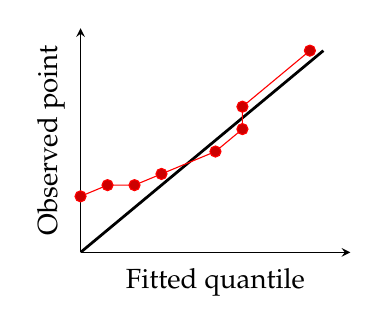
\begin{tikzpicture}
        \begin{axis}[
            scale=0.5,
            axis x line=bottom,
            axis y line=left,
            xtick=\empty,
            ytick=\empty,
            xlabel={Fitted quantile},
            ylabel={Observed point},
            xlabel near ticks,
            ylabel near ticks,
            xmin = 0,
            xmax = 10,
            ymin = 0,
            ymax = 10]
            \addplot[mark=none, draw=black, line width=1pt] coordinates {%
                  (0,0) (9,9)
            };
            \addplot+[mark=*, draw=red] coordinates {%
                  (0,2.5) (1,3) (2,3) (3,3.5) (5,4.5) (6,5.5) (6,6.5) (8.5,9)
            };

        \end{axis}
    \end{tikzpicture}
\end{center}

\def\SectionColor{blue!80!white}
\section*{Lesson 42: Introduction to Extended Linear Models}
There are two purposes in building a extended linear model.
\begin{enumerate}[align=left,leftmargin=*]
  \item \textbf{Prediction:} We want to predic the valu of the \emph{response} variable given specific values of the \emph{explanatory} variables.
  \item \textbf{Inference:} We want to understand which \emph{explanatory} variables explain the \emph{response} variable and how much their explain it.
\end{enumerate}
To evaluate the accuracy of a model, we estimate it mean square error.
\[\hspace*{0.5cm} \mathrm{MSE} = \frac{1}{n} \sumn (y_i - \hat{y}_i) \]
% \vspace{10cm}
\columnbreak
\section*{Lesson 43: How a Generalized Linear Model Works}
\begin{itemize}[align=left,leftmargin=*]
  \item \textbf{Linear Model:} \\
  $\hspace*{0.5cm} Y = \eta + \varepsilon =  \beta_0 + \beta_1 x_1 + ... + \beta_p x_p + \varepsilon $
  \item[] where
  \begin{align*}
    \hspace*{1cm}
    \varepsilon &\sim N(0, \sigma^2) \\
    Y &\sim N(\eta, \sigma^2)
  \end{align*}
  \textbf{Hypothesis}:
  \begin{itemize}
    \item[($\mathbf{H_1}$)] $\esp{\varepsilon} = 0\quad\quad\quad\quad\:$(Linearity)
    \item[($\mathbf{H_2}$)] $\var{\varepsilon} = \sigma^2\quad\quad\:\:\:\:$(Homoscedasticity)
    \item[($\mathbf{H_3}$)] $\covar{\varepsilon_i, \varepsilon_j} = 0\quad$(Independence)
  \end{itemize}
  \item The \textbf{Box-Cox transformation} is a general set of transformation. When the variance of the error terms is not constant($\mathrm{H_2}$), we need to transforme $Y$.
  \[ \hspace*{0.5cm}
  Y^{*} = \left\{
  \begin{array}{lr}
    \frac{Y^\lambda - 1}{\lambda} & \lambda \neq 0 \\
    \ln Y & \lambda = 0
  \end{array}
  \right.
  \]
  \item[] where $\lambda$ is chossen to best stabilize the variance of the error terms.
  \item The \emph{feature} must be linearly independent. That mean their can't be a function of another. Ex: $X_3 = 1 - X_2$.
  \item We need to encode categorials variables with $k$ levels into ($k-1$) indicators variables(called \emph{dummy} variables) to avoid \emph{feature} to be dependent. For interaction with 2 categorials variables, ($k-1$)($l-1$) dummy variables are needed.
  \item \textbf{GLM:} \\
  $\hspace*{1cm} g(\esp{Y}) = \beta_0 + \sumn \beta_i x_i$
  \item[] where g($\cdot$) is the link function.
  \item \textbf{Exponential Family:} \\
  $\hspace*{0.7cm} f(y;\theta) = \mathrm{exp}\{a(y)b(\theta) + c(\theta) + d(y)\}$
  \item[] with
  \begin{align*}
    \hspace*{0.2cm}
    \esp{a(y)} &= -\frac{c'(\theta)}{b'(\theta)} \\
    \var{a(y)} &= \frac{b''(\theta)c'(\theta) - c''(\theta)b'(\theta)}{[b'(\theta)]^3}
  \end{align*}
  \item \textbf{Tweedie} distribution: \\
  $\hspace*{2cm}  \var{Y} = a\esp{y}^p$
  \item \textbf{link function:} The GLM estimate is unbiased when the canonical link is used.
  \begin{center}
    \begin{tabular}{ll}
    \hline
    Distribution & Canonical link \\
    \hline
    Normal & $g(y) = y$ \\
    Binomial & $g(y) = \ln \frac{y}{1-y}$ \\
    Poisson & $g(y) = \ln y$ \\
    Gamma &  $g(y)=\frac{1}{y}$ \\
    \hline
    \end{tabular}
  \end{center}
  \item \textbf{Offset:} We add $\ln n_i$ for cell with $n_i$ exposure.
  \item \textbf{Rate ratio:} \\
  $\hspace*{2cm} RR = \frac{\esp{Y_i|x_j = 1}}{\esp{Y_i|x_j = 0}}$
\end{itemize}
\columnbreak

\section*{Lesson 44: Categorial \\ Response}
\subsubsection*{Binomial Response}
\begin{itemize}[align=left,leftmargin=*]
  \item Let $\pi_i\in(0,1)$  be the response variable. We than need to have link that map $\eta$ into $(0,1)$.
  \begin{itemize}
    \item \textbf{logit:} $ \ln\left(\frac{\pi}{1-\pi}\right) = \eta$
    \item \textbf{Probit:} $ \Phi^{-1}(\pi) = \eta$
    \item \textbf{Log-log:} $\ln(-\ln(1-\pi)) = \eta$
  \end{itemize}
  \item \textbf{Odds Ratio:} $o = \frac{\pi}{1 - \pi}$
\end{itemize}
\subsubsection*{Nominal Response}
\begin{itemize}[align=left,leftmargin=*]
  \item Suppose the response can be $J$ values. Then we create a model of relative odds. \\
  $\hspace*{1cm}\ln \frac{\pi_j}{\pi_1} = \eta_j \Leftrightarrow \pi_j = \pi_1e^{\eta_j}$
  \begin{itemize}
    \item $\pi_i = \frac{1}{1 + \sum_{j=2}^J e^{\eta_j}}$
    \item $\pi_j = \frac{e^{\eta_j}}{1 + \sum_{j=2}^J e^{\eta_j}}$
  \end{itemize}
  \item If $x_i$ is a binary feature, then the odds ratio of this \textbf{variable} in the category $j$ to the base categorie is $e^{\beta_{ij}}$.
\end{itemize}
\subsubsection*{Ordinal Response}
Ordinal response variables have several categories in logical order.
\begin{itemize}[align=left,leftmargin=*]
  \item \textbf{Cumulative logit and proportional odds models:}
  \begin{align*}
    o_j = \ln \frac{\sum_{k=1}^j \pi_k}{1-\sum_{k=1}^j \pi_k} = \eta_j
  \end{align*}
  Tips: The model is cumulative, so to find $\pi_{2}$, we need to find $\pi_{1}$ and $\pi_{1}+\pi_{2}$. \\
  This model is proportional so if we $\textbf{fix}$ the categorie but consider two set of feature $x_{i1}$ and $x_{i2}$, the relative odds are \\
  $\hspace*{1cm} \frac{(o_j|x_i=x_{i1})}{(o_j|x_i=x_{i2})} = e^{\sum \beta_i (x_{i1} - x_{i2})}$
  \item \textbf{Adjacent categorie logit model:}  \\
  \begin{align*}
    \hspace*{1cm}
    \ln \frac{\pi_j}{\pi_{j+1}} &= \eta_j \\
    \sum_{j=1}^J \pi_j &= 1
  \end{align*}
  \item \textbf{Continuation ratio logit model:} \\
  \hspace*{0.5cm}
    $\ln \frac{\pi_j}{\sum_{k=j+1}^J \pi_k} = \ln \frac{\pi_j}{1 - \sum_{k=1}^j \pi_k} = \eta_j$ \\
    Tips: Resolve for $\pi_1$ then for $\pi_2$ and so on ...
\end{itemize}
\columnbreak

\section*{Lesson 45: Estimating Parameters}
\begin{itemize}[align=left,leftmargin=*]
  \item Let $\matr{X}$ be the \textbf{design matrix}, the p x n features matrix.
  \item \textbf{Linear Regression:} \\
  \begin{align*}
    \hat{\beta}_1 &= \frac{\sum x_iy_i - n\bar{x}\bar{y}}{\sum x_i^2 - n\bar{x}^2} \\
    \hat{\beta}_0 &= \bar{y} - \hat{\beta}_1 \bar{x} \\
    \matr{b} &= (\matr{X}^\intercal\matr{X})^{-1}\matr{X}^\intercal \matr{y}
  \end{align*}
  \item The \textbf{score} function is define as the derivative of the loglikehood \\
  $\hspace*{2cm} \matr{U}(\beta) = \ell'(\beta)$
  \item \textbf{Newton-Raphson} algorithm: \\
  $\hspace*{1.5cm} \beta^{(k+1)} =\beta^{(k)} - \frac{\matr{U}(\beta^{(k)})}{\matr{U}'(\beta^{(k)})}$
  \item \textbf{Fisher Scoring} algorithm:\\
  $\hspace*{1.5cm} \beta^{(k+1)} =\beta^{(k)} - \frac{\matr{U}(\beta^{(k)})}{\esp{\matr{U}'(\beta^{(k)})}}$
  \item The score vector has components \\
  $\hspace*{1cm} U_j =\sumn \frac{y_i - \mu_i}{\var{y_i}}x_{ij}\left( \frac{\diff g(\mu_i)}{\diff \mu_i}\right)$
  \item The information matrix: $I(\theta) = \matr{X}^\intercal\matr{W}\matr{X}$
  \item Let $\matr{W}$ be the diagonal matrix with entries \\
  $\hspace*{1.5cm}w_{ii} =\left( \left(\frac{\diff g(\mu_i)}{\diff\mu_i}\right)^2 \var{y_i}\right)^{-1}$
  \item Let $\matr{G}$ be the diagonal matrix with entries \\
  $\hspace*{2cm}G_{ii} =\frac{g(\mu_i)}{\mu_i}$
  \item The regression variable for one iteration \\
  $\hspace*{0.5cm}\matr{z}^{(k-1)}= \matr{X}\matr{b}^{(k-1)} + \matr{G}^{(k-1)}(\matr{y} - \matr{\mu}^{(k-1)})$
  \item The \textbf{Weighted Least Square}: \\
  $\hspace*{0.5cm} \matr{b}^{(k)} = (\matr{X}^\intercal\matr{W}^{(k-1)}\matr{X})^{-1}\matr{X}^\intercal\matr{W}^{(k-1)}\matr{z}^{(k-1)}$
\end{itemize}

\section*{Lesson 46: Measures of Fit}
\begin{itemize}[align=left,leftmargin=*]
  \item The \textbf{satured} model is when we have as much feature as parameters($p=n$). $g^{-1}(\matr{X}^\intercal\matr{b}) = \matr{y}$
  \item The \textbf{deviance} statistic test compare a model to the satured model. \\
  $\hspace*{1cm} D = 2[\ell(\matr{b}_{max}) - \ell(\matr{b})] \approx n - p'$
  \item[] where $p'=p+1$ and $p$ the number of feature.
  \begin{itemize}
    \item Binomial:\\
    $D = 2 \sumn \left(y_i \ln \frac{y_i}{\hat{y}_i} + (n_i - y_i)\ln \frac{n_i - y_i}{n_i - \hat{y}_i} \right)$
    \item Normal (\emph{scaled deviance}): \\
    $\sigma^2 D = \sumn (y_i - \hat{y}_i)^2$
    \item Poisson: \\
    $D = 2\sumn \left(y_i \ln \frac{y_i}{\hat{y}_i} - (y_i - \hat{y}_i) \right)$
    \item Gamma: \\
    $D = 2 \alpha \sumn \left(-\ln \frac{y_i}{\hat{y}_i} + \frac{y_i - \hat{y}_i}{\hat{y}_i} \right)$
  \end{itemize}
\end{itemize}
\columnbreak
\subsubsection*{Signifiance of Feature}
\begin{itemize}[align=left,leftmargin=*]
  \item \textbf{Loglikehood ratio test:} These tests compare a \textbf{unconstrained} modele with $p+q$ parameters versus another \textbf{constrained }model with $p$ parameters. \\
  $\hspace*{1.5cm} H_0: \mathrm{Model}p+q)$ \\
  $\hspace*{1.5cm} H_1: \mathrm{Model}(p)$ \\ 
  $\hspace*{1.5cm} 2(\tilde{\ell}_{p+q} - \hat{\ell}_p) \sim \chi_{(q)}^2$\\
  $\hspace*{2cm} \hat{D} - \tilde{D} \sim \chi_{(1)}^2$
  \item \textbf{Wald test:} To test wheter a single parameter $\beta_j=r$. \\
  $\hspace*{1.7cm} W = \frac{(\hat{\beta}_j - r)^2}{\var{\hat{\beta}_j}} \sim \chi_{(1)}^2$
  \item[] $\sqrt{W} \sim N(0,1)$, is usefull for confidence interval.
  \item[] $I(\theta)^{-1} = (\matr{X}^\intercal\matr{W}\matr{X})^{-1}$ is the covariance matrix.
  \item \textbf{Score text:} $ \matr{U}^\intercal I(\theta)^{-1}\matr{U}\sim \chi_{(q)}^2$
  \item[] If $q=1,\; \frac{U}{\sqrt{I(\theta)}}\sim N(0,1).$
  \item We want the lowest AIC and BIC.
\end{itemize}

\section*{Lesson 47: Standard Error, $R^2$, and Strudent Statistic}
$\hspace*{2cm} SST = SSE + SSR$
\begin{itemize}[align=left,leftmargin=*]
  \item \textbf{Total sum of square:} $SST = \sumn (y_i - \bar{y})^2$
  \item \textbf{Error sum of square:} $SSE = \sumn (y_i - \hat{y}_i)^2$ \\
  $\hspace*{1cm} SSE = \matr{\varepsilon^\intercal\varepsilon} = \matr{y}^\intercal\matr{y} - \matr{b}^\intercal\matr{x}^\intercal\matr{y} $
  \item \textbf{Regression sum of square:} $SSR = \sumn (\hat{y}_i - \bar{y})^2$
\end{itemize}
\begin{center}
  \begin{tabular}{cccc}
    \hline
    \multicolumn{4}{c}{ANOVA} \\
    \hline
    SS & df & MS & F \\
    \hline
    SSR & p & MSR = SSR/df & $\frac{MSR}{MSE}$\\
    SSE & n-p' & MSE = SSE/df &\\
    SST & n-1 & MST = SST/df &\\
    \hline
  \end{tabular}
\end{center}
\begin{itemize}[align=left,leftmargin=*]
  \item The standort error of the regression is \\
  $\hspace*{2cm}  s=\sqrt{MSE}$
  \item The \textbf{coefficient of determination} is the proportion explain by the regression. \\
  $\hspace*{1.2cm} R^2 = \frac{SSR}{SST} = 1 - \frac{SSE}{SST}$
  \item \textbf{Strudent test:} To test $\beta_i = \beta^*$\\
  $\hspace*{2cm} t_{n-p'} = \frac{\beta_i - \beta^*}{S_{\beta_i}}$
  \item[] Matrice variance-covariance: $\sigma^2(\matr{X}^\intercal\matr{X})^{-1}$
  \item Simple linear regression:
  \begin{itemize}
    \item $\var{\hat{\beta}_0} = \sigma^2 \left(\frac{1}{n} + \frac{\bar{x}^2}{S_{xx}} \right)$
    \item $\var{\hat{\beta}_1} = \frac{\sigma^2}{S_{xx}}$
    \item $\covar{\hat{\beta}_0, \hat{\beta}_1} = -\frac{\bar{x}\sigma^2}{S_{xx}}$
  \end{itemize}
\end{itemize}
\columnbreak

\section*{Lesson 48: Fisher Statistic and VIF}
\begin{itemize}[align=left,leftmargin=*]
  \item The \textbf{Fisher} statistic test the signifiance od the entire regression, in other word if all $\beta_i = 0$. For simple linear regression $F = T^2$.
  Tips: Divide numerator and denominator of $F$ by SST to find $R^2$.
  \item For simple linear regression, since $p=1$, then \\
  $\hspace*{2cm} T_{(n)} = \sqrt{F_{1,n}}$.
  \item \textbf{Partial Fisher test:} To test is $q$ added variables have signifiance. \\
  $\hspace*{1cm} F_{\Delta_{df},n-p'} = \frac{SSE^{(0)} - SSE^{(1)}/\Delta_{df}}{SSE^{(1)}/(n-p')}$
  \item The \textbf{Variance Inflation Factor} test the collinearity of the features. To mesure it, we take the $x_j$ feature and take it as the response. Let $R_{(j)}^2$ be the $R^2$ of this regression. \\
  $\hspace*{2cm} \textrm{VIF} = \frac{1}{1 - r_{(j)}^2}$
  \item[] We want the lowest VIF.
  \item \textbf{Coeficient of correlation:} \\
  $\hspace*{1cm} r = \frac{\covar{X,Y}}{\sigma_x \sigma_y} = \frac{\sum (x_i-\bar{x})(y_i - \bar{y}) }{\sqrt{\sum (x_i-\bar{x})^2 \sum (y_i - \bar{y})^2}}$
  \item For two-feature model $R_{(y)}^2 = r^2$.

\end{itemize}

\section*{Lesson 49: Validation} 
\begin{itemize}[align=left,leftmargin=*]
   \item The \textbf{Hat matrix} put a hat on $y$ since $\hat{\matr{y}} = \matr{H}\matr{y}$. \\
   $\hspace*{2cm} \matr{H} = \matr{X}(\matr{X}^\intercal\matr{X})^{-1}\matr{x}^\intercal$
   \item It follow that $\var{\hat{\varepsilon}} = (\matr{I} - \matr{H})\sigma^2$
   \item For simple linear regression: \\
   $\hspace*{2cm}h_{ii} = \frac{1}{n} + \frac{(x_i - \bar{x})^2}{S_{xx}}$
   \item The \textbf{studentized residuals} are define as \\
   $\hspace*{2cm} r_i = \frac{\hat{\varepsilon}_i}{\sqrt{S^2(1 - h_{ii})}}$
   \item[] where $h_{ii}$ is the \textbf{leverage}. Average leverage should be at $\frac{p'}{n}$.$\quad \sum h_{ii} = p'$
   \item A \textbf{influence point} is a observatio that influence a lot $y$. A \textbf{outliers} is a observation that have $|r_i|>3$. 
   \item Two mesure for influence point.
   \begin{itemize}
      \item $\mathrm{DFITS}_i = r_i \sqrt{\frac{h_{ii}}{1- h_{ii}}}$
      \item \textbf{Cook:} $D_i =\frac{\sum (\hat{y}_j - y_{j(i)})^2}{p^{'}S^2} =r_i^2 \frac{h_{ii}}{p'(1 - h_{ii})}$
      \item[] $D_i>1$ is too high. 
   \end{itemize}
 \end{itemize} 
 
\section*{Lesson 50: Prediction}
\begin{itemize}[align=left,leftmargin=*]
    \item A \textbf{confidence interval} for predicted values. \\
    $\hspace*{0.5cm}y^{*} \in \hat{y}^{*} \pm t_{(n-2)} \sqrt{S^2\left(\frac{1}{n}+\frac{(x^{*} - \bar{x})^2}{S_{xx}}\right)}$
    \item A \textbf{prediction interval} for predicted values. \\
    $\hspace*{0.5cm}y^{*} \in \hat{y}^{*} \pm t_{(n-2)} \sqrt{S^2\left(1+\frac{1}{n}+\frac{(x^{*} - \bar{x})^2}{S_{xx}}\right)}$
\end{itemize}
 
\section*{Lesson 51: ANOVA}
\subsubsection*{One-factor ANOVA}
$\hspace*{2cm} \mathrm{SST} = \mathrm{SSE} + \mathrm{SSTR}$
   \begin{center}
      \begin{tabular}{lcc}
        \hline
        Model & Sum of square & Deviance \\
        \hline
         $Y = \mu + \varepsilon_{ij}$ & SST & $D_M$ \\
         $Y = \mu_i + \varepsilon_{ij}$ & SSE & $D_A$ \\
         \hline
      \end{tabular} 
   \end{center} 
\begin{itemize}[align=left,leftmargin=*]
   \item  \textbf{Within sum of square} \\
   $\hspace*{1cm} \mathrm{SSE} = \sum\limits_{i=1}^k \sum\limits_{j=1}^{n_i} (y_{ij} - \bar{y}_{i\Sigma})^2$
   \item \textbf{Between sum of square} \\
   $\mathrm{SSTR} = \sum\limits_{i=1}^k n_i (\bar{y}_{i\Sigma} - \bar{y}_{\Sigma\Sigma})^2 = \sum\limits_{i=1}^k \left(\frac{y_{i\Sigma^2}}{n_i}\right)  - n\bar{y}_{\Sigma\Sigma}^2$
   \item \textbf{Total sum of square} \\
   $\mathrm{SST} = \sum\limits_{i=1}^k \sum\limits_{j=1}^{n_i} (y_{ij} - \bar{y}_{\Sigma\Sigma})^2 = \sum\limits_{j=1}^{n_i} (y_{ij}^2) - n\bar{y}_{\Sigma\Sigma}^2$ \\
   \item \textbf{Fishier test} \\
   $F_{(k-1, n-k)} = \frac{\mathrm{SSTR}/(k-1)}{\mathrm{SSE}/(n-k)} = \frac{(D_M - D_A)/(k-1)}{D_A/(n-k)}$
   \item[] where $D_M$ is the \emph{scale deviance} of the minimal model.
\end{itemize}
\subsubsection*{Two-factor ANOVA without replication}
$\hspace*{1.5cm} \mathrm{SST} = \mathrm{SSE} + \mathrm{SSTR} + \mathrm{SSB}$
   \begin{center}
      \begin{tabular}{ll}
        \hline
        Model & Sum of square (DF) \\
        \hline
         $Y = \mu + \varepsilon_{ij}$ & SST$(bk-1)$  \\
         $Y = \mu + \alpha_i + \varepsilon_{ij}$ & SSTR $(k-1)$ \\
         $Y = \mu + \beta_j + \varepsilon_{ij}$ &SSB$(b-1)$ \\
         $Y = \mu +\alpha_i +  \beta_j + \varepsilon_{ij}$ & SSE$(k-1)(b-1)$  \\
         \hline
      \end{tabular} 
   \end{center} 
\begin{itemize}[align=left,leftmargin=*]
  \item The formula are the same but $n_i$ is $k$ for SSTR and $b$ for SSB. 
\end{itemize}
\subsubsection*{Two-factor ANOVA with replication}
\begin{itemize}[align=left,leftmargin=*]
   \item To test interaction:\\
   $F_{(I-1)(J-1),IJ(K-1)} = \frac{(D_I - D_s)/(I-1)(J-1)}{D_s/IJ(k-1)}$ 
   \item To test factor A:\\
   $F_{(I-1),IJ(K-1)} = \frac{(D_B - D_I)/(I-1)}{D_s/IJ(k-1)}$ 
   \item To test factor B: \\
   $F_{(J-1),IJ(K-1)} = \frac{(D_M - D_B)/(J-1)}{D_s/IJ(k-1)}$ 
   \item[] where $D_s$ is the satured model, I for additive model.
   \item ANCOVA
\end{itemize}


\section*{Lesson 52: Measures of Fit II}
For \textbf{contingencies table}  with binomial or poisson distribution.
\begin{itemize}[align=left,leftmargin=*]
%    \item Deviance: $D = 2 \sum O_i \ln \frac{O_i}{E_i}$ 
   \item Pearson: $\chi^2 = \sum \frac{(O_i - E_i)^2}{E_i} \sim \chi_{(n-p')}^2$
   \item Likelihood ratio chi-square: \\ $\hspace*{1.5cm} C = 2[\ell - \ell_{\mathbf{min}}] \sim \chi_{(p'-1)}^2$
   \item \textbf{Pseudo}$R^2$: $\mathrm{pseudo}R^2 = 
   \frac{\ell_{\mathbf{min}} -  \ell}{\ell_{\mathbf{min}}}$
\end{itemize}
\subsubsection*{Residus}
\begin{itemize}[align=left,leftmargin=*]
   \item Pearson residual: $X_k = \frac{y_i - \hat{\mu}_i}{\sqrt{\var{\hat{\mu}_i}}}$
   \item Deviance residual: $d_k = s_k\sqrt{\mathrm{deviance}}$ 
   \item[] where $s_k$ is the signe of $y_k-\hat{y}_i$
   \item To standartize them, divide by $\sqrt{1-h_{ii}}$
\end{itemize}


\section*{Lesson 53: Resampling Methods}
\begin{itemize}[align=left,leftmargin=*]
   \item \textbf{Cross-Validation:}\\
  $\hspace*{1.5cm}  \mathrm{CV}_{(K)} = \frac{1}{k} \sum\limits_{i=1}^k MSE_i $ 
  \item[] If $k=n$ then is the $\mathrm{LOOCV}$ statistic.
  \item $\mathrm{LOOCV}$ for least-square regression: \\
  $\hspace*{1.5cm} \mathrm{CV}_{(K)} = \frac{1}{n} \sum_{i=1}^n \left( \frac{\varepsilon_i}{1-h_{ii}}\right)^2$
  \item \textbf{Bootstap:} \\
  $\hspace*{1.5cm} \mathrm{SE}_B(\alpha) = \sqrt{\frac{1}{1-B} \sum\limits_{i=1}^B (\hat{\alpha} - \bar{\alpha})^2}$
\end{itemize}

\section*{Lesson 54: Subset Selection}
Using a lot of feature will result of lower standard error on training data, but poor prediction. We need to keep only the feature that truly impact the response.
\begin{itemize}[align=left,leftmargin=*]
   \item \textbf{Subset selection} For $k$ possible feature, $2^k$ different model are possible.
   \begin{itemize}
    \item For 2 model with same number of feature, we take the one with lowest $SSE$.
    \item Otherwise, we compare with: Mallow's $C_p$, AIC, BIC and adjusted $R^2$.
   \end{itemize}
   \item \textbf{Foward stepwise selection} consist of starting with the null, then fit $k$ models with one variable and select the best base on SSE, then fit $k-1$ variables and so on. We obtain $k+1$ model, the best for each number of predictor, and select the final one with cross-validation or the 4 statistics. For categorial variables, each categorie is added independently.
   \item \textbf{Total fitted model:} 
   \begin{itemize}
      \item Foward: $1 + \sum\limits_{i=0}^{\min(p,n)} (\min(p,n) - i)$ 
      \item Backward: $1 + \sum\limits_{i=1}^{\min(p,n)} i$
   \end{itemize}
\end{itemize}
\subsubsection*{Choosing the best model}
\begin{itemize}
   \item \textbf{Cross-validation} is the more accurate.
   \item \textbf{Mallow's $\mathbf{C_p}$:} $C_p = \frac{1}{n}(SSE + 2p\hat{\sigma}^2)$ 
   \item[] IF $\hat{\sigma}^2$ is unbiased then $C_p$ is unbiased.
   \item \textbf{Adjested $\mathbf{R^2}$:} $R_a^2 = 1 -  \frac{MSE}{MST}$
   \item We want the lowest Mallow's $C_p$, AIC, BIC and the heighest $R_a^2$.
\end{itemize}

\section*{Lesson 55: Shrinkage and Dimension Reduction}
\begin{itemize}[align=left,leftmargin=*]
   \item  \textbf{Ridge Regression:} Minimize \\
   $\hspace{1cm} \left(\sumn y_i - \beta_0 - \sum\limits_{j=1}^{p'-1} \beta_j x_{ij}\right) + \lambda \sum\limits_{j=1}^{p'-1} \beta_j^2$
   \item \textbf{Lasso Regression:} Minimize \\
   $\hspace{1cm} \left(\sumn y_i - \beta_0 - \sum\limits_{j=1}^{p'-1} \beta_j x_{ij}\right) + \lambda \sum\limits_{j=1}^{p'-1} |\beta_j|$
   \item \textbf{Standart Predictors} $\tilde{x} = \frac{x_{ij}}{\sqrt{\frac{1}{n}\sum (x_{ij}-\bar{x})^2}}$
   \begin{align*}
      \lambda &\to \infty \Leftrightarrow \beta_j \to 0 \\
      \lambda &\to 0 \Leftrightarrow \beta_j \to \hat{\beta}_j^{\mathrm{normal}}
   \end{align*}
\end{itemize}
\begin{tabular}{l|l}
    \hline
   PCA & Partial Least Square \\
   \hline
   unsupervised & supervised \\
   \multicolumn{2}{c}{variables are linear combianaire of the original} \\
   Higher bias & Lower bias \\
   Lower variance & Higher variance  \\
   \hline 
\end{tabular}

\section*{Lesson 56:Extension to the Linear Model}
\begin{itemize}[align=left,leftmargin=*]
   \item \textbf{Extention:} These type can be treate as same as GLM. $y_i = \beta_0 + \beta_1 b_1(x_i) + \beta_2 b_2(x_i) + ... + \varepsilon_i$
   \item[] For \textbf{polynomial regression}, $b_j(x) = x^j$.
   \item[] For \textbf{piecewise constant regression} \\ $ b_j(x) = \indic{a\leq x<b}(x) $
   \item \textbf{Generalized Additive Model:} \\
   $\hspace*{1cm} y_i = \beta_0 + \sum_{j=1}^p f_i(x_{ij}) + \varepsilon_i$
   \begin{itemize}
      \item Allows nonlinear fits for each explanatory variable.
      \item Effet on each explanatory is separate, so easily identifiable.
      \item Does not allow foe effect of interaction among variable. 
   \end{itemize}
\end{itemize}


\def\SectionColor{green!80!black}
\section*{Lesson 57: Trend and \\Seasonality}
\begin{itemize}[align=left,leftmargin=*]
  \item \textbf{Trend} measures the amount by which the serie increase from period to period.
  \item \textbf{Seasonal} variation measure cycle within a year.  
  \item \textbf{Decomposition models}
  \begin{itemize}
     \item  Additive Model: $x_t = m_t + s_t + z_t$
     \item Multiplicative Seasonality: $x_t s_t + z_t$
     \item Multiplicative Model: $x_t = m_t s_t z_t$
  \end{itemize}
  \item \textbf{Centered moving average:} \\
  $\hat{m}_t = \frac{0.5m_{t-k} + m_{t-k+1} + ... + m_t + ... + m_{t+k-1} + 0.5m_{t+k}}{2k}$
  \item \textbf{Seasonal variation factor:}  
  \begin{itemize}
     \item Additive Seasonality: $\hat{s}_t = x_t - \hat{m}_t$
     \item[] Ajusted so that $\sum (s_t + c) = 0$.
     \item  Multiplicative Seasonality $\hat{s}_t = \frac{x_t}{\hat{m}_t}$
     \item[] Ajusted so that $\sum \frac{(\hat{s}_t + c)}{n}= 1$.
  \end{itemize}
\end{itemize}

\section*{Lesson 58: correlation}
\begin{itemize}[align=left,leftmargin=*]
    \item if $\mu(t) $ and $\sigma^2(t)$ does not vary with $t$ then the time serie is \textbf{second order stationnary}
   \item \textbf{Variance:} $\sigma^2(t) = \esp{(x_t -       \mu(t))^2}$
\end{itemize}
\subsubsection*{Stationnary Time serie}
\begin{itemize}[align=left,leftmargin=*]
    \item \textbf{sample variance} $s^2 = \frac{1}{n-1} \sumn (x_t - \bar{x})^2$
    \item \textbf{Covariance} at lag $k$ : \\
    $\covar{x_t,x_{t+k}} = \gamma_k = \esp{(x_t - \mu)(x_{t+k} - \mu)} \: (\textbf{acvf}) $
    \item[] $c_k = \frac{1}{n} \sum_{i=1}^{n-k} (x_t - \bar{x})(x_{t+k} - \bar{x})\quad (\textbf{sample acvf})$
    \item \textbf{Auto-correration} \\
     $\rho_k = \frac{\covar{x_t,x_{t+k}}}{\sigma^2}\quad (\textbf{acf})$ \\
    $r_k = \frac{c_k}{c_0}\quad (\textbf{sample acf})$
\end{itemize}
\subsubsection*{Relationships of different time serie}
\begin{itemize}[align=left,leftmargin=*]
   \item A \textbf{leading variable} is one that impact another.   
   \item \textbf{Cross-covariance} \\
    $\gamma_k(x,y) = \esp{(x_{t+k} - \mu_x)(y_t - \mu_y)} \quad (\textbf{ccvf}) $
    \item[] $c_k = \frac{1}{n} \sum\limits_{i=1}^{n-k} (x_{t+k} - \bar{x})(y_t - \bar{y})\quad (\textbf{sample ccvf})$
    \item \textbf{Cross-correration} \\
     $\rho_k(x,y) = \frac{\gamma_k(x,y)}{\sigma_x \sigma_y}\quad (\textbf{ccf}) $ \\
    $r_k = \frac{c_k(x,y)}{\sqrt{c_0(x,x)c_0(y,y)}}\quad (\textbf{sample ccf})$
    \item Notice
    \begin{align*}
      \gamma_k(x,y) &= \gamma_{-k}(x,y) \\
      \rho_k(x,y) &= \rho_{-k}(x,y) \\
       c_0(x,x) &= c_0
    \end{align*}
\end{itemize}

\section*{Lesson 59: White Noise and Random Walks}
\begin{itemize}[align=left,leftmargin=*]
   \item \textbf{White noise} each term are independant and variance $\sigma^2$. The correlogram has autocorrelations all close to 0 except for $r_0$. \\
   $\hspace*{1.5cm} w \sim N(0,\sigma^2) $
   \item A \textbf{Random Walks} is a nonstationary time series which is the accumulation of white noise. The correlogram will decrease slowly from 1 to 0.
   $\hspace*{2cm}x_1 = w_1$ \\
   $\hspace*{2cm}x_t = x_{t-1} + w_t$
   \item[] with 
   \begin{align*}
        \hspace*{1cm}
      \mu(t) &= 0 \\
      \sigma^2(t) &= t\sigma_w^2 \\
      \gamma_k(t) &= t\sigma_w^2 \\
      \rho_k(t) &= \frac{1}{\sqrt{1 + \frac{k}{t}}}
   \end{align*} 
   \item A \textbf{Walk with drift} drift the mean $\mu(t) = t\delta$ by don't affect variance and autocorrelations.
   $\hspace*{2cm} x_t = x_{t-1} + \delta + w_t$ 
\end{itemize}

\section*{Lesson 60: Autoregressive Models}
\begin{itemize}[align=left,leftmargin=*]
    \item An \textbf{autoregressive} model of order ($p$), or AR(p) is a time series where term may be expressed in term of previous terms plus white noise.
    \begin{align*}
    x_t - \mu =& \alpha_1(x_{t-1} - \mu) + \alpha_2(x_{t-2} - \mu) \\ 
    +& ...  + \alpha_p(x_{t-p} - \mu) + w_t
    \end{align*}
    \item An AR(1) process is stationary if $|a|<1$. correlogram is deacreasing exponentially. For a stationary AR(1) process \\
    \begin{align*}
    \hspace*{1cm}
      \mu_k &= 0 \\  
      \gamma_k &= \frac{\alpha^k \sigma_w^2}{1 - \alpha^2} \\
      \rho &= \alpha^k
    \end{align*}
    \item Notation: $\matr{B}^kx_t = x_{t-k}$
    \begin{align*}
        w_t &= x_t - \alpha_1 x_{t-1} - \alpha_2 x_{t-2}\\
        &= (\alpha_2\matr{B}^2 - \alpha_1\matr{B} + 1)x_t \\
        &= \theta_p(\matr{B})x_t
    \end{align*}
    \item[] where $\theta_p(\matr{B})$ is the \textbf{characterictic equation}. 
    \item Testing stationarity: Root $< 1$
    \item[(given)] $x_t = \alpha_1 x_{t-1} + \alpha_2 x_{t-2} + w_t$
    \item[(solve)] $\theta_p(\matr{B}) = 0$  
    \item[(answer)] If $|\matr{B}| > 1$, the process is stationary.
    \item tips: For 2 param:
    \begin{align*}
        \hspace*{1cm}
       \alpha_2 - \alpha_1 < 1 \\
       \alpha_2 + \alpha_1 < 1 \\
       |\alpha_2| < 1 
    \end{align*}
    \item Forecast $\hat{x}_{n+1|n}$ is the same equation omitting $w_t$.
\end{itemize}

\section*{Lesson 61: Regression}
\begin{itemize}[align=left,leftmargin=*]
    \item Variance of sample mean with correction is given by \\ $\var{\bar{x}} = \frac{\sigma^2}{n} \left(1 + 2\sum\limits_{k=1}^{n-1} \left(1 - \frac{k}{n}\right)\rho_k\right)$
    \item \textbf{Harmonic Seasonal model}\\
    $x_t = m_t + \sum_{i=1}^{[S/2]} s_i \sin(2\pi i t/s) $\\
    $\hspace*{1cm}+ c_i \cos(2\pi i t/s) + z_t$
    \item Forecast correction
    \begin{itemize}
       \item Lognormal: $e^{\sigma^2/2}$ 
       \item Empirical: $\frac{\Sigma e^{z_t}}{n}$
    \end{itemize}
\end{itemize}

\section*{Lesson 62: Moving Average Models}
\begin{itemize}[align=left,leftmargin=*]
   \item A \textbf{moving average} time serie (MA(q)) is alway stationary. It define as \\ 
    $x_t = \mu + w_t + \beta_1 w_{t-1} + ... + \beta_q w_{t-q}$ \\ 
    $\hspace*{0.35cm}= \mu + \phi(\matr{B})w_t$ 
    \item[] with 
    \begin{align*}
      \mu(t) &= 0 \\  
       \gamma_k &= \sigma_w^2 \sum_{i=0}^{q-k} \beta_i \beta_{i+k}\quad \beta_0 = 1\\
    \end{align*} 
    \item[] and $\gamma_k = 0$ for $k>q$ so MA(q) may be good fit is we observe $\gamma_q = 0$ in correlogram.
    \item $q$ beta + $\mu$ + $\sigma_w^2 = q+2$ parameters fit.
    \item A MA(q) is \textbf{Inversible} if all the root of 
    $ \phi(\matr{B})$ are $|\matr{B}|>1$
    \item Express MA(q) in form of AR($\infty$). If $ \phi(\matr{B})$ is reversible: \\
    $\frac{1}{1+x} = 1 - x + x^2 - x^3 + x^4 + ..$\\
    $\frac{1}{1-x} = 1 + x + x^2 + x^2 + x^4 + ...$
    \item ARIMA with $p = d = 0$ is a MA(q) model.
    \item conditional sum of squared residuals: $\sum w_t^2$
\end{itemize} 


\section*{Lesson 63: ARMA Models}
\begin{itemize}[align=left,leftmargin=*]
   \item The ARMA(p,q) models:\\
   $x_t = \alpha_1 x_{t-1} + ... + \alpha_p x_{t-p} + \beta_1 + w_{t-1} + ... + \hspace*{0.35cm} \beta_q w_{t-q} + w_t$
   \item[] $\theta_p(\matr{B})x_t = \phi_q(\matr{B})w_t$
   \item The process is stationary if all roots of $\theta(x)>1$ and the process is inversible if all roots of $\phi(x)>1$
   \item[]
    \begin{align*}
      \gamma_0 &= \sigma_w^2 \left(\frac{1 + 2\alpha\beta + \beta^2}{1 - \alpha^2} \right)  \\
      \gamma_k &= \sigma_w^2 (\alpha + \beta) \alpha^{k-1}\left(\frac{1+\alpha\beta}{1 - \alpha^2}\right)
    \end{align*}
    \item[] $\rho_k = \alpha\rho_{k-1}$ for $k\geq2$.
    \item If the process is stationary, $\esp{x_t} = \esp{x_{t-1}}$. 
\end{itemize}

\section*{Lesson 64: ARIMA and SARIMA models}
\begin{itemize}[align=left,leftmargin=*]
    \item $\triangledown x_t + x_t - x_{t-1} = (1 - \matr{B})x_t$
   \item An \textbf{ARIMA} model is a nonstationary process. If $x_t$ is an ARIMA model, then $y_t = \triangledown^d x_t$ is an ARMA(p,q). Then the ARIMA(p,d,q) is \\
   $\hspace*{1cm} \theta(\matr{B})(1-\matr{B})^d x_t = \phi(\matr{B})w_t$
   \begin{itemize}
     \item With no MA(q), this is ARI(p,d)
     \item With no AR(p), this is IMA(d,q)  
   \end{itemize}
   \item An \textbf{SARIMA} model is a ARIMA with seasonal effect.
   \item To forecast, we take the difference and then forecast ARMA(p,q) model.
\end{itemize}



 % -------------------------------------
 % Appendix 
 % ------------------------------------- 
\part*{Appendix}
\def\SectionColor{black!80!white}
\section*{Inverting a matrix}
\label{Appendix: Inverting a matrix}
\begin{align*}
    \hspace*{-0.9cm}
    \begin{pmatrix}
            a & b \\
            c & d
        \end{pmatrix}^{-1}
    =
    \frac{1}{ad-bc}
    \begin{pmatrix}
            d & -b \\
            -c & a
    \end{pmatrix}
\end{align*}



\hl{Ajouter pour une matrice 3x3}

\section*{Synthetic Division}
\label{Appendix: Synthetic Division}
\textbf{Exemple:} Factorize $x^3 - 12x^2 - 81$\\
\begin{tabular}{c|cccc}
     & 1 & -12 & 0 & -81 \\
   3 &   &   3 & -27& -81 \\
   \hline
     & 1 & -9  & -27  & 0
\end{tabular} \\
then, $x^3 - 12x^2 - 81 = (x-3)(x^2-9x-27)$

\section*{Deductible and Limite}
\begin{align*}
    X &= \min(X;d) + \max(0;X-d) \\
    \esp{X} &= \esp{\min(X;d)} + \esp{\max(0;X-d)} \\
            &= \esp{(X \wedge d)} + \esp{(x-d)_{+}} \\
            &= \esp{(X \wedge d)} + e_x(d)\cdot S_x(d)
\end{align*}

\section*{Statistic Order}
\label{Appendix: Statistic Order}
\begin{itemize}[align=left,leftmargin=*]
    \item $Y_1 = \min(X_1, ... ,X_n)$
    \begin{align*}
        f_{Y_1}(y) &= nf(y)[S(y)]^{n-1} \\
        S_{Y_1}(y) &= \prod_{i=1}^n \prob{X_i>x}
    \end{align*}
    \item $Y_n = \max(X_1, ... ,X_n)$
    \begin{align*}
        f_{Y_n}(y) &= nf(y)[F(y)]^{n-1} \\
        F_{Y_n}(y) &= \prod_{i=1}^n \prob{X_i\leq x}
    \end{align*}
    \item $Y_k \in (Y_1,...,Y_k,...,Y_n)$
    \begin{align*}
        f_{Y_k}(y) &= \frac{n!\cdot f(y)[F(y)]^{k-1}[S(y)]^{n-k}}{(k-1)!(n-k)!} \\
        F_{Y_k}(y) &= \prob{\text{at least k of n $X_i$ are $\leq$ y}} \\
                   &= \sum_{i=k}^n \binom{n}{i} [F(y)]^i[S(y)]^{n-j}
    \end{align*}
    \item $x+y=\min(x,y)+\max(x,y)$, since one is for sure the max and the other the min.
\end{itemize}

\section*{Mode: Most likely \\ probability}
\begin{itemize}[align=left,leftmargin=*]
    \item $g(x) = f(x)$ or some time $g(x) = \ln f(x)$
    \item \textbf{Mode} is the $x$ that respects: $g'(x) = 0$
\end{itemize}

\section*{Normal Approximation}
\begin{itemize}[align=left,leftmargin=*]    
    \item $F_X(x) = \Phi \left( \frac{X - \esp{X}}{\sqrt{\var{X}}} \right)$
    \item \textbf{Continuity correction} is necessary when X is discrete. $F_X(x) = \Phi \left( \frac{(X \pm k) - \esp{X}}{\sqrt{\var{X}}} \right)\:$ where $k$ is the mid-point of the discrete value.
\end{itemize}

\section*{Discrete Cumulative Function}
\label{Appendix: Discrete Cumulative Function}
\begin{align*}
    \prob{X = x} &=
    \left\{
        \begin{array}{cl}
            0.10, & x = 0 \\
            0.30, & x = 5 \\
            0.15, & x = 10 \\
            0.25, & x = 15 \\
            0.20, & x = 20 \\
        \end{array}
    \right. \\
    \prob{X \leq x} &=
    \left\{
        \begin{array}{cc}
        0.10, & 0 \leq x < 5 \\
        0.40, & 5 \leq x < 10 \\
        0.55, & 10 \leq x < 15 \\
        0.80, & 15 \leq x < 20 \\
        1, & x \geq 20 \\
        \end{array}
    \right.
\end{align*}
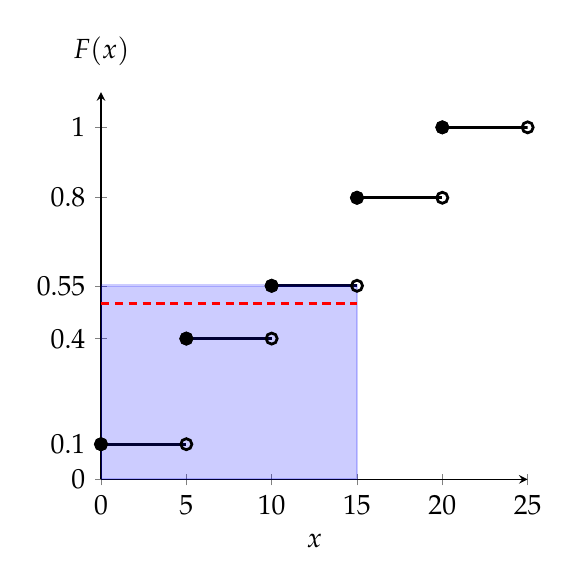
\begin{tikzpicture}
    \begin{axis}[
        height=6.5cm,
        width=7cm,
        axis x line=bottom,
        axis y line=left,
        xlabel = {$x$},
        title = {\hspace*{-5.5cm} $F(x)$},
        ytick={0, 0.10, 0.40, 0.55, 0.80, 1},
        xmin = 0,
        xmax = 25,
        ymin = 0,
        ymax = 1.1]
        \addplot[mark=o, draw=black, line width=1pt] coordinates { (0,0.1)(5,0.1) };
        \addplot[mark=o, draw=black, line width=1pt] coordinates { (5,0.4)(10,0.4) };
        \addplot[mark=o, draw=black, line width=1pt] coordinates { (10,0.55)(15,0.55) };
        \addplot[mark=o, draw=black, line width=1pt] coordinates { (15,0.8)(20,0.8) };
        \addplot[mark=o, draw=black, line width=1pt] coordinates { (20,1)(25,1) };

        \addplot[mark=*, draw=black, line width=1pt] coordinates { (0,0.1) };
        \addplot[mark=*, draw=black, line width=1pt] coordinates { (5,0.4) };
        \addplot[mark=*, draw=black, line width=1pt] coordinates { (10,0.55) };
        \addplot[mark=*, draw=black, line width=1pt] coordinates { (15,0.8) };
        \addplot[mark=*, draw=black, line width=1pt] coordinates { (20,1) };

        \addplot[mark=none, draw=blue, line width=1pt, fill=blue, opacity=0.2] coordinates { (0,0.55)(15,0.55) }\closedcycle;
        \addplot[mark=none, draw=red, line width=1pt, densely dashed] coordinates { (0,0.50)(15,0.50) };

        \draw (45,25) node[right]{$F^{-1}(0.50) = 10$};
    \end{axis}
\end{tikzpicture}

\section*{Contract}
\begin{itemize}[align=left,leftmargin=*]
    \item \textbf{Deductible(d)}
    \item \textbf{Maximum(u)}
    \item \textbf{Inflation(r)}
    \item \textbf{Coinsurance($\boldsymbol{\alpha}$)}
\end{itemize}
\begin{align*}
    Y &=
    \left\{
        \begin{array}{cc}
        0 & x \leq \frac{d}{1+r}\\
        \alpha[(1+r)x-d] & \frac{d}{1+r} < x < \frac{u}{1+r} \\
        \alpha[u - d] & x \geq \frac{u}{1+r} \\
        \end{array}
    \right.
\end{align*} \\
{\color{red} Warning: The maximal don't include the deductible.}

\section*{Moments}
\begin{itemize}[align=left,leftmargin=*]
    \item k\up{e} moment about the origin. $\mu_k'=\esp{X^k}$
    \item k\up{e} moment about the mean. $\mu_k=\esp{(X-\mu)^k}$
    \item The \textbf{Skewness} moment give infomation about the asymmetry of the distribution. If $S_{sk}=0$, the distribution is normal. \[\hspace*{1cm} S_{sk} = \esp{\left(\frac{X-\mu}{\sigma^2}\right)^3} \] %If $S_{sk}=0$, the distribution is normal.
    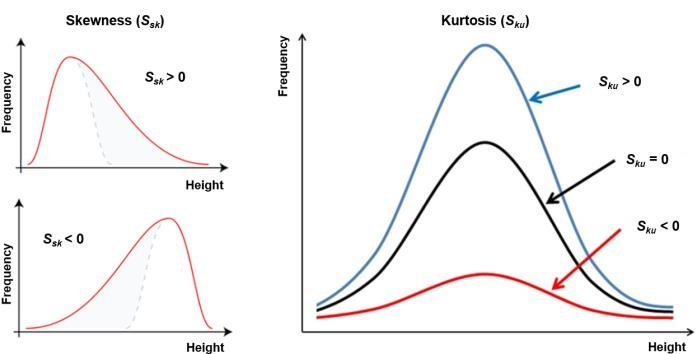
\includegraphics[scale=0.34]{src/Illustration-skewness-and-kurtosis.png}
    \item The \textbf{kurtosis} moment give infomation about the flattening of the distribution. If $S_{ku}=0$, the distribution is normal. \[\hspace*{1cm} S_{ku} = \esp{\left(\frac{X-\mu}{\sigma^2}\right)^4} \] %If $S_{ku}=0$, the distribution is normal.
    \item The \textbf{coefficient of variation} give information about the dispersion of the distribution. \[\hspace*{1.1cm} \mathrm{CV} = \frac{\sigma}{\esp{X}} \]
\end{itemize}

\section*{Transformations of distribution}
\label{Appendix: Transformations distribution}
\begin{itemize}[align=left,leftmargin=*]
    \item Lognormal: $Y = e^{X}$, where
    \begin{align*}
        Y &\sim \mathrm{Lognormal}(\mu, \sigma) \\
        X &\sim \mathrm{Normal}(\mu, \sigma)
    \end{align*}
    \item Inverse Exponential: $Y = \frac{1}{X}$, where
    \begin{align*}
        Y &\sim \mathrm{Inverse\:Exponential}(1/\theta) \\
        X &\sim \mathrm{Exponential}(\theta)
    \end{align*}
    \item Weibull: $Y = X^{1/\tau}$, where
    \begin{align*}
        Y &\sim \mathrm{Weibull}(\sqrt[\tau]{\theta}) \\
        X &\sim \mathrm{Exponential}(\theta)
    \end{align*}
\end{itemize}

\section*{Parameter interpretation}
\begin{itemize}[align=left,leftmargin=*]
    \item \textbf{Scale parameter ($\theta$, $\beta$, $\sigma$):} Affect the spread of the distribution.
    \item \textbf{Rate parameter ($\lambda$):} Affect the rate of data at mean. (1/scale)
    \item \textbf{Shape parameter ($\alpha$, $\tau$, $\gamma$):} Affect the shape rather then simply shift the distribution.
\end{itemize}

\section*{Produit de convolution}
The convolution of 2 random variable is difine as the sum of the two. \\
\begin{align*}
  f_{X_1+X_2}(x) &= \int_{-\infty}^\infty f_{X_1}(x - s)f_{X_2}(s)\diff{s} \\
  F_{X_1+X_2}(x) &= \int_{-\infty}^x F_{X_1}(x - s)f_{X_2}(s)\diff{s}
\end{align*}

\section*{Shifting Exponential}
\begin{align*}
   f(x;\theta;d) &= \frac{1}{\theta} e^{-(x-d)/\theta} \\
   \esp{x}&= \theta + d \\
    \var{x} &= \theta^2    
\end{align*}

\section*{Norme d'un vecteur}
\begin{align*}
   \ell_1 &= x_1 + x_2 + ... + x_n \\
   \ell_2 &= \sqrt{x_1^2 + x_2^2 + ... + x_n^2}
\end{align*}

\section*{Greedy algorithm}
A group of $n$ peoples is to be assigned to $k$ job, one to each job. The cost of job j is $c_{ij}$ if person i is assigned.
Select the assignement to have the minimal cost. 
\begin{align*}
   c_{ij} &\sim \mathrm{Exp}(\theta) \\
   \esp{\textbf{Total cost}} &= \sum \min(c_{11} + ... + c_{1n} + ... + c_{kn}) \\
   \esp{\textbf{Total cost}} &= \frac{\theta}{n\cdot k} + \frac{\theta}{(n-1)\cdot(k-1)} + ... 
\end{align*}

\end{multicols*}
%% -----------------------------
%% Fin du document
%% -----------------------------
\end{document}
